\documentclass[msc,numbers]{coppe}
\usepackage[utf8]{inputenc}
\usepackage{amsmath,amssymb, mathtools}
\usepackage{hyperref}
\usepackage{indentfirst}
\usepackage{graphics}
\usepackage{float}
\usepackage{algpseudocode,algorithm}
%%%%%%%%%%%%%%%%%%%%%%%%%%%%%%%%%%%%%%%%%%%%%%%%%%%%%%%%%%%%%%%%%%%%%%%%%%%%%%%%%%%%%%%%%%%%%%%%
% Modificado por Geraldo Xexéo
% para permitir entender melhor as citações
%% Bibliografia
\usepackage{natbib}
\setcitestyle{authoryear,open={(},close={)}}
\bibliographystyle{coppe-plain}
% Declarações em Português do Pseudocódigo
\algrenewcommand\algorithmicend{\textbf{fim}}
\algrenewcommand\algorithmicdo{\textbf{faça}}
\algrenewcommand\algorithmicwhile{\textbf{enquanto}}
\algrenewcommand\algorithmicfor{\textbf{para}}
\algrenewcommand\algorithmicforall{\textbf{para cada}}
\algrenewcommand\algorithmicif{\textbf{se}}
\algrenewcommand\algorithmicthen{\textbf{então}}
\algrenewcommand\algorithmicelse{\textbf{senão}}
\algrenewcommand\algorithmicreturn{\textbf{devolve}}
\algrenewcommand\algorithmicfunction{\textbf{função}}
\algrenewtext{EndWhile}{\algorithmicend\ \algorithmicwhile}
\algrenewtext{EndFor}{\algorithmicend\ \algorithmicfor}
\algrenewtext{EndIf}{\algorithmicend\ \algorithmicif}
\algrenewtext{EndFunction}{\algorithmicend\ \algorithmicfunction}
\algnewcommand\algorithmicto{\textbf{até}}
\algrenewtext{For}[3]%
{\algorithmicfor\ #1 $\gets$ #2 \algorithmicto\ #3 \algorithmicdo}
\makeatletter
\newcommand{\newalgname}[1]{%
  \renewcommand{\ALG@name}{#1}%
}
\newalgname{Algoritmo}% All algorithms will be called "Algoritmo"
\renewcommand{\listalgorithmname}{Lista de \ALG@name s}
\makeatother
%%%%%%%%%%%%%%%%%%%%%%%%%%%%%%%%%%%%%%%%%%%%%%%%%%%%%%%%%%%%%%%%%%%%%%%%%%%%%%%%%%%%%%%%%%%%%%%%
\newcommand{\argmin}{\arg\!\min}
\newcommand{\argmax}{\arg\!\max}
\newcommand*\rfrac[2]{{}^{#1}\!/_{#2}}

\makelosymbols
\makeloabbreviations

\begin{document}
  \title{titulo}
  \foreigntitle{titulo em ingles}
  \author{nome}{sobrenome}
  \advisor{Prof.}{nome orientador}{sobrenome}{D.Sc.}
  %\advisor{Prof.}{segundo orientador}{sobrenome}{D.Eng.}
  %\advisor{Prof.}{Nome do Terceiro Orientador}{Sobrenome}{D.Sc.}

  \examiner{Prof.}{Nome do primeiro Examinador Sobrenome}{D.Sc.}
  \examiner{Prof.}{Nome do segundo Examinador Sobrenome}{D.Sc.}
  \examiner{Prof.}{Nome do terceiro Examinador Sobrenome}{D.Sc.}
  \examiner{Prof.}{Nome do Quarto Examinador Sobrenome}{Ph.D.}
  %\examiner{Prof.}{Nome do Quinto Examinador Sobrenome}{Ph.D.}
  \department{PESC}
  \date{mes}{ano}

  \keyword{}
  \keyword{}
  \keyword{}
  
  %\abbrev{SR}{Sistema de Recomendação}
  %\abbrev{AM}{Aprendizado de Máquina}
  %\abbrev{AA}{Aprendizado Ativo}

  \maketitle

  \frontmatter
  \dedication{Soli Deo Gloria}


  \chapter*{Agradecimentos}

Em toda caminhada longa e árdua, há momentos de tropeço e desânimo que só são superados quando alguém lhe estende a mão e lhe coloca novamente no caminho. No meu caso não foi diferente, portanto, tenho muitas mãos a agradecer.

Agradeço ao meu orientador, prof. Geraldo Zimbrão, por acreditar no meu potencial e pela orientação deste trabalho. Minha gratidão aos membros da banca pelo tempo e atenção devotados à análise desta dissertação. Em especial, ao prof. Carlos Mello, cujas ideias e conselhos foram fundamentais, não apenas em minha vida acadêmica, mas também em minha vida pessoal. Cadu, se assim me permite, meu muito obrigado.

Quero agradecer aos meus amigos do PESC, que, entre um café e outro, me deram dicas de leitura; apontaram meus erros; apludiram meus acertos; me deram caronas; me contaram piadas; escutaram pacientemente minhas angústias e alegrias. Braida, Duarte, Horta, Luis e Pedro, não sei se aguentaria sem vocês.

Não posso deixar de agradecer ao prof. Daniel Figueiredo que, desde da graduação, me motivou a entrar no mundo acadêmico e, durante o mestrado, sempre se mostrou solicito a escutar meus problemas e pensar em soluções. Agradeço também a todos os funcionários do PESC e da CAPES por proverem uma infraestrutura onde pude me apoiar.

Sem dúvida, o maior auxílio que tive foi o amor e suporte da minha família. Não só agradeço, como também dedico este trabalho a eles: meus pais, minha irmã, meus avós, meus tios e primos. Meu muito obrigado pelo carinho; pelas palavras de ternura; pela compreensão e pelos tantos ``vai dar tudo certo''.

Por último, mas não menos importante, agradeço à mão que me pôs de pé após as quedas mais dolorosas e angustiantes. Obrigado Deus, por tudo!
  \begin{abstract}

resumo

\end{abstract}


  \begin{foreignabstract}

abstract

\end{foreignabstract}


  \tableofcontents
  \listoffigures
  \listoftables
  \listofalgorithms
  \addcontentsline{toc}{chapter}{\listalgorithmname}
  \printlosymbols
  \printloabbreviations
  %\addcontentsline{toc}{chapter}{\listabbreviationname}

  \mainmatter
  \chapter{Introdução}
\section{Motivação}

Há uma frase, de autor desconhecido, mas que ficou muito famosa, com o dizer: ``informação é o novo petróleo''. Apesar do conteúdo sensacionalista, não é possível negar que a veracidade da mesma vem se confirmando nas últimas décadas. De fato, nunca se produziu tanta informação em toda história e, ao mesmo tempo, nunca se dependeu tanto da mesma. As maneiras habituais de trabalho, estudo, locomoção, relacionamento e convívio foram completamente remodeladas, passando a ser fortemente informatizadas. Ou seja, os indivíduos estão cada vez mais dependentes de aparatos tecnológicos para executar tarefas antes consideradas básicas e triviais. Tal fenômeno chamou a atenção dos pesquisadores que o batizaram de \textit{Era da Informação} \citep{castells_information_1999}.

Existem muitas vantagens e desvantagens associadas à tal Era da Informação, assim como em tudo o mais. No entanto, uma de suas mais aclamadas vantagens está se transformando em uma desvantagem. Boa parte desta sobrecarga de informação se encontra atualmente na Internet, o que cria uma enorme oferta de opções para os usuários. A intuição comum normalmente associa variedade à satisfação, isto é, quanto mais opções um usuário tiver, consequentemente, mais satisfeito ele estará. Contudo, o que se observa na prática é que, frente a um demasiado numero opções, os usuários se angustiam, uma vez que o risco de fazer a escolha errada aumenta consideravelmente. Portanto, a exacerbada variedade de opções vem causando descontentamento ao invés de satisfação \citep{schwartz_paradox_2004}.

Este paradoxo torna-se mais visível quando consideramos o comércio eletrônico, também conhecido como \textit{e-commerce}. Uma das esferas da vivência humana mais afetada pela Era da Informação foi, sem dúvida, o comércio. Chega a ser difícil encontrar uma empresa que não oferte seus produtos \textit{online}. Por outro lado, a Internet deixou de ser apenas mais um canal de comunicação com o cliente e passou a ser o habitat natural de novos negócios, muitos deles comercializando bens intangíveis (e.g., \textit{software}, áudio, vídeo, etc.), que são facilmente armazenáveis. Some-se a isto o fato de que as lojas virtuais, quando ofertam bens tangíveis, isto é, produtos físicos em geral, não precisam tê-los em estoque no momento da venda. Tais fatores conferem aos \textit{e-commerces} uma enorme flexibilidade para montar seus catálogos, que podem atingir facilmente a ordem de milhões de itens.

Comprar, por sua vez, nunca foi uma ação tão simples e, ao mesmo tempo, tão complexa. Simples no sentido de que a revolução informacional acabou criando formas mais eficientes de pagamentos e, hoje, é possível literalmente comprar uma grande quantidade de itens com apenas um \textit{click}. Entretanto, escolher o que comprar se tornou uma tarefa complexa tendo em vista as inúmeras possibilidades oferecidas \textit{online}. O usuário comum se depara com uma infinidade de lojas virtuais, de toda parte do globo, cada uma com um catálogo praticamente ilimitado de itens. Não é atoa que estão surgindo diversos serviços voltados somente para auxiliar o usuário a encontrar o que deseja, como, por exemplo, buscadores específicos para produtos, comparadores de preço, atendimento virtual, entre outros.

Dentre as ferramentas que visam auxiliar o usuário durante a compra, nenhuma chamou tanto a atenção da indústria quanto os Sistemas de Recomendação (SR). Durante as últimas duas décadas, as grandes empresas da Internet investiram fortemente em tais sistemas, pois perceberam que o usuário se sente perdido em meio a tantas opções e, no fim, acaba por desistir da compra. Ao oferecer recomendações, o sistema pretende amenizar a dúvida do usuário, reduzindo o número de opções a se considerar. Ademais, a loja virtual passa a sensação de que compreende o usuário, ou seja, que sabe distinguir entre os itens que ele gosta e os que ele não gosta. 

%\abbrev{SR}{Sistema de Recomendação}

Além de, claro, aumentar a probabilidade de venda ao recomendar os itens que o usuário gosta (ou pelo menos que o site acredita que ele gosta), a sensação de ser atendido de forma personalizada estabelece, em muitos usuários, uma relação de confiança. Em outras palavras, SR não servem apenas para alavancar vendas, podem ser concebidos como uma forma de se estreitar o relacionamento com o cliente \citep{Schafer:1999:RSE:336992.337035}.

A academia, por sua vez, também investiu com veemência no aprimoramento das técnicas de recomendação. Em especial, a competição organizada pelo \textit{Netflix} trouxe muita atenção para este tema, uma vez que levou pesquisadores de todo o mundo a trabalharem em um algoritmo que fosse mais eficiente que o do próprio \textit{Netflix} \citep{Bennett07thenetflix}. Como resultado, diversos algoritmos foram propostos, a grande maioria se baseando em métodos de Aprendizado de Máquina (AM) e Data Mining (DM), o que trouxe importantes avanços para a área \citep{Bell:2007:LNP:1345448.1345465, ricci_recommender_2011}.

%\abbrev{AM}{Aprendizado de Máquina}
%\abbrev{DM}{Data Mining}

Em geral, as técnicas de recomendação podem ser divididas em três abrangentes categorias: Baseadas em Contexto (BC), Filtragem Colaborativa (FC) e Híbridas. No capítulo \ref{cap:fundamentacao}, iremos descrever em detalhes cada uma dessas categorias e as principais técnicas de cada uma. Por hora, é suficiente mencionar que as técnicas de FC se sobressaem às demais, principalmente em termos de desempenho e aplicabilidade. No entanto, elas sofrem com o problema do \textit{Arranque Frio} (AF), ou problema do \textit{Novo Usuário/Item}. Como muitas delas se baseiam em noções de similaridade entre usuários/itens, extraídas a partir das preferências dos usuários, não é possível calcular nenhuma recomendação para o novo usuário/item, visto que não se pode medir sua similaridade para com os demais usuários/itens \citep{su_survey_2009}.

%\abbrev{FC}{Filtragem Colaborativa}
%\abbrev{AF}{Arranque Frio}

Por esta razão, muitos trabalhos foram propostos na tentativa de amenizar o problema do AF em FC, sobretudo no tocante ao novo usuário \citep{Rashid:2002:GKY:502716.502737, Rashid:2008:LPN:1540276.1540302, elahi_rating_2011, elahi_system-wide_2011, Elahi:2014:ALS:2542182.2542195}. Tais propostas buscam aumentar o conhecimento do sistema sobre os novos usuários, solicitando aos mesmos que deem suas preferências (na forma de avaliações) para alguns itens previamente definidos. A este processo, que precede o cálculo das recomendações, damos o nome de \textit{Elicitação de Preferências}.

É importante delinear que a Elicitação de Preferências pode ser utilizada em contextos que não são necessariamente relacionados ao problema de AF. Infelizmente, na literatura, esses termos podem parecer sinônimos, uma vez que a grande maioria dos trabalhos envolvendo Elicitação de Preferências são voltados para contornar as deficiências geradas pelo AF. A fim de distinguir os cenários onde o processo de elicitação pode ser aplicado, iremos denominar o caso referente ao AF como \textit{Elicitação de Preferências para fins de Arranque Frio}.

\section{Proposta}

Avaliar não é um hábito comum para boa parte dos usuários, de forma que, na maioria das lojas virtuais, sabe-se apenas quem comprou o que. Informações sobre a preferência dos usuários é difícil de se obter, visto que não há um incentivo direto para que eles avaliem os itens que compraram. Claro que muitos contribuem com suas preferências na esperança de poder ajudar os que estão em dúvida sobre um determinado item; outros simplesmente porque gostam de deixar seu contentamento (ou seu desprezo) registrados como forma de gratidão (ou revolta) para com o fornecedor; e há ainda aqueles que entendem que o sistema depende das preferências para calcular as recomendações e, por isto, contribuem na esperança de melhorar a qualidade das mesmas.

Em todo o caso, a motivação para contribuir com as suas preferências possui sempre aspectos colaborativos, visando o ganho do sistema, ou de outros usuários, e nunca o ganho individual. Embora tenham ocorrido mudanças significativas, sobretudo na \textit{Web}, em direção a maior colaboração entre os usuários, o simples espírito altruísta parece não ser suficiente para mobilizar a maioria, que continua não contribuindo assiduamente. Enquanto boa parte dos trabalhos que se propõem a motivar os usuários acabam por enveredar pela via colaborativa, tentando maximizá-la \citep{Carenini:2003:TMC:604045.604052, ling_using_JCC4, Rashid:2006:MPD:1124772.1124915}, outros foram além e procuraram pensar em um modelo econômico que capturasse a maneira como os usuários dão suas preferências \citep{harper_economic_2005, market_avery_1999}. Em \citep{lee2013alleviating}, os autores procuram elicitar preferências da multidão, usando incentivos, na esperança de que isto melhore o desempenho das técnicas de FC. Como não é possível saber quais itens são avaliáveis, \citep{lee2013alleviating} acaba tratando da \textit{Elicitação de Preferências para fins de Arranque Frio} no contexto de multidão.

%Desta maneira, seria possível propor mecanismos de incentivo a ``produção de preferências'' similares aos incentivos governamentais a produção de bens de consumo, por exemplo. Todavia, ambas abordagens pecam no mesmo ponto, isto é, ambas tratam todas as preferências como possuindo a mesma importância, ou valor, para o SR.

Uma vez que tais sistemas possuem a informação de compra, isto é, sabem quem comprou o que, é razoável assumir que, se um usuário comprou um determinado item, logo, ele é capaz de avaliar este item. Esta suposição não se dá necessariamente de forma imediata, pois certos itens requerem uma quantidade significativa de tempo para serem ``consumidos'' (e.g., livros e filmes). Contudo, o que podemos assumir é que, dado que um usuário efetuou a compra de um item, passado um determinado intervalo de tempo, este usuário estará apto a dar sua preferência sobre o item em questão, seja ela boa ou ruim.

Ao solicitar que o usuário avalie um item que ele já comprou, a probabilidade de se obter uma preferência, em forma de avaliação, é muito maior do que quando o mesmo é solicitado a avaliar um item a esmo. Portanto, temos aqui o outro contexto onde o processo de Elicitação de Preferências se encaixa bem, isto é, elicitar as preferências sobre itens já comprados. É importante ressalvar que nada impede que o processo de elicitação seja aplicado concomitantemente tanto neste caso quanto no caso voltado para o AF. O que chama a atenção sobre este contexto é o fato dele ser até mais eficiente na aquisição de preferências do que no primeiro caso. A \textit{Amazon}, por exemplo, tenta persuadir seus clientes a contribuírem com suas preferências enviando \textit{emails}, tempos após a compra, contendo os itens comprados e a opção de avaliá-los \citep{linden_amazon_2003}.

No só a \textit{Amazon}, mas praticamente todas as lojas virtuais procuram elicitar as preferências a respeito dos itens comprados pelo usuário, este fato, em si, não é nenhuma novidade. Geralmente, o processo de elicitação se dá através do envio de \textit{emails} ou alguma outra forma de notificação. Todavia, se os \textit{e-commerces} solicitarem que cada usuário avalie todos os itens já comprados, poderão gerar um excesso de notificações que causará incômodo aos usuários. Infelizmente, na prática, é exatamente isto o que acontece e, o pior, os usuários mais incomodados são justamente aqueles que mais compram, ou seja, os melhores clientes. Este erro ocorre devido a uma suposição muito questionável, a de que todas as preferências contribuem da mesma forma para o SR. É muito plausível que certas preferências possuam maior impacto no desempenho do SR que outras, assim poderíamos obter um ganho equivalente, ou até mesmo superior, solicitando menos notificações aos clientes, o que lhes pouparia paciência.

Tanto neste caso como no caso referente ao AF, há um problema em comum no tocante a como selecionar os itens que devem ser avaliados por cada usuário. Nos trabalho voltados para a \textit{Elicitação de Preferências para fins de Arranque Frio}, os itens a se avaliar são escolhidos através de estratégias de Aprendizado Ativo (AA). Tais técnicas surgiram como uma subárea dentro de AM e visam selecionar as ``melhores'' instâncias de modo a construir o menor e mais eficaz conjunto de treinamento possível. Ou seja, estratégias de AA possibilitam que os modelos de AM sejam treinados de maneira mais rápida, tornando-os mais precisos com menos esforço de treinamento. No cenário referente a SR, a técnica de recomendação e as preferências podem ser considerados modelo de AM e instâncias de treinamento, respectivamente. Um apanhado geral sobre as diversas estratégias de AA pode ser encontrado no capítulo \ref{cap:fundamentacao}

%\abbrev{AA}{Aprendizado Ativo}

Supondo que o \textit{e-commerce} saiba quais são os $N$ itens que, se avaliados pelo usuário, irão trazer o maior ganho possível para o SR, em termos de desempenho, o mesmo pode oferecer ao usuário um incentivo individual a fim de garantir que este contribua com suas preferências. Como exemplo de incentivo pessoal, podemos citar desconto em futuras compras; pontos a serem trocados pro brindes ou vales; \textit{upgrade} no tipo de conta; entre outros. É importante frisar que a escolha dos incentivos que serão implantados e como os mesmos serão implantá-los foge a nossa \textit{expertise}, visto que se trata de um problema de administração ou de economia. Entretanto, a tarefa de encontrar os $N$ itens a serem avaliados por cada usuário pode ser atacada através de estratégias de AA. Este trabalho propõe portanto o emprego de tais estratégias a fim de se encontrar os $N$ itens mais importantes para cada usuário avaliar. A importância dessas preferências para o desempenho do SR deve ser tamanha a ponto do sistema estar disposto a oferecer incentivos individuais ao usuário pelas mesmas. Convencionamos chamar este problema de \textit{Elicitação de Preferências para fins de Incentivo}.

Mais ainda, uma das principais deficiências das estratégias de AA é o fato de que todas se baseiam em suposições sobre os dados, i.e., heurísticas. Quando estas suposições não se verificam na prática, as estratégias acabam por gerar um conjunto de treinamento enviesado, algo que, ao invés de impulsionar, prejudica o desempenho do sistema. Em suma, a qualidade das recomendações depende diretamente da estratégia empregada pelo SR, logo é vital que os projetistas saibam escolher aquela que trará o maior ganho para o sistema. 

Para não cairmos na problemática relacionada ao viés, propomos o emprego de uma nova estratégia. A batizada \textit{Estratégia Livre de Viés} ainda é desconhecida pela literatura relacionada a SR, sendo este trabalho sua primeira utilização em tal contexto. Como veremos no capítulo \ref{cap:estrategia-livre-vies}, esta estratégia busca selecionar os itens de forma a aproximar a Função de Distribuição de Probabilidade (FDP) dos mesmos, garantindo que o conjunto de treinamento gerado é o que melhor representa a totalidade dos dados, i.e., sem viés. 

Realizamos uma extensa comparação entre as estratégias de AA, em duas bases de dados consideradas clássicas na literatura. Ao todo, foram comparadas 17 estratégias, incluindo a \textit{Estratégia Livre de Viés}, e verificou-se que esta última, em ambas as bases, supera as demais. O desempenho de cada estratégia foi analisado no capítulo \ref{cap:resultados}, onde explicamos o motivo do sucesso ou fracasso das mesmas considerando as características das bases de dados. Mesmo havendo estratégias que possuem desempenho próximo a \textit{Estratégia Livre de Viés}, acreditamos ter encontrado uma excelente opção para todos os tipos de bases.

\section{Contribuições}

As contribuições deste trabalhos podem ser resumidas aos itens abaixo:

\begin{itemize}

\item Introdução do problema referente a \textit{Elicitação de Preferências para fins de Incentivo}, que não foi devidamente explorado na literatura até então.
\item Emprego de uma estratégia nunca antes utilizada no contexto de SR, a \textit{Estratégia Livre de Viés}, que garante produzir um conjunto de treinamento sem viés.
\item Realização do experimento mais completo da literatura, envolvendo ao todo 17 estratégias, incluindo a \textit{Estratégia Livre de Viés}.
\item Analise do desempenho, seja ele bom ou ruim, de cada estratégia, levando em consideração as características da base de dados.
\end{itemize}

\section{Organização}

Esta dissertação está organizada em 6 capítulos, dos quais este é o primeiro. No capítulo \ref{cap:fundamentacao}, iremos descrever os principais conceitos teóricos envolvidos, além de mencionar os trabalhos relacionados ao tema. No capítulo \ref{cap:estrategia-livre-vies}, detalharemos como funciona a \textit{Estratégia Livre de Viés} e como a mesma foi adaptada ao problema de SR. No capítulo \ref{cap:metodologia}, apresentamos a metodologia que guiou nossos experimentos, bem como as demais estratégias comparadas. No capítulo \ref{cap:resultados}, expomos os resultados obtidos e iniciamos uma investigação tentando encontrar os motivos por trás do sucesso ou fracasso de cada estratégia. Finalmente, no capítulo \ref{cap:conclusao}, tiramos as devidas conclusões e apontamos possíveis trabalhos futuros.
  \chapter{Fundamentação Teórica}
\label{cap:fundamentacao}

\section{Sistemas de Recomendação}
Sistemas de Recomendação (SR) surgiram como uma área de pesquisa independente em meados da década de 90, quando foram desenvolvidos os primeiros sistemas de filtragem baseados nas preferências dos usuários como o \textit{Tapestry} \citep{Goldberg:1992:UCF:138859.138867}, o \textit{Ringo} \citep{Shardanand:1995:SIF:223904.223931} e o \textit{GroupLens} \citep{Resnick:1994:GOA:192844.192905}. Até este momento, o problema de recomendação era considerado como um caso específico de filtragem de informação e, portanto, era tratado dentro da área de Recuperação de Informação (RI) \citep{Baeza-Yates:1999:MIR:553876}. A partir de então, a área devotada a SR cresceu de maneira considerável, devido a enorme aplicabilidade que esses sistemas possuem no cenário econômico atual.

Um dos trabalhos mais completos desta área, \citep{Adomavicius:2005:TNG:1070611.1070751} define SR através de uma função de utilidade $u(i,j)$ que exprime a importância, ou o valor, que o item $j$ possui para o usuário $i$. As avaliações dos usuários são consideradas observações da função de utilidade no espaço de usuários e itens. Assim, cabe ao SR tentar estimar artificialmente $u$ para os pontos do espaço onde não há observação. 

Em termos formais, seja $U$ o conjunto de todos os usuários do sistema e $I$ o conjunto de todos os itens do sistema. Em aplicações atuais de \textit{e-commerce}, ambos podem chegar facilmente a ordem de milhões elementos. A função de utilidade a ser estimada é tal que $u: U \times I \rightarrow \mathbb{N}$ ou $u: U \times I \rightarrow \mathbb{R}$, dependendo do tipo de avaliação dada pelos usuários. Desta forma, um SR visa encontrar, para cada usuário $i$, o item $j'$ tal que: 

\begin{equation}
\forall i \in U, \quad j' = \argmax_{j \in I} u(i,j) 
\end{equation}

Uma vez encontrado o item, ou conjunto de itens, que maximiza a função de utilidade para um determinado usuário, o SR pode então recomendá-lo ao usuário, na esperança de que o mesmo o adquira. Ou seja, no caso de um \textit{e-commerce}, o sistema procura os itens que maximizam a probabilidade do usuário efetuar a compra.

O espaço de usuário e itens $U \times I$ é, na prática, representado por uma matriz conhecida como matriz de preferências. Um exemplo de tal matriz pode ser visto na tabela \ref{tab:preferencias}, onde os usuários estão dispostos em linhas e os itens em colunas. Cada posição $r_{ij}$, dada pela interseção da linha $i$ com a coluna $j$, contem a preferência do usuário $i$ pelo item $j$ em forma de nota. Vale ressaltar que, quando o usuário não explicita sua preferência a respeito do item, a posição $r_{ij}$ da matriz fica em aberto, o que é representado pelo símbolo $\varnothing$. Como normalmente cada usuário avalia um subconjunto muito pequeno de itens, a grande maioria das posições na matriz de preferências são do tipo $\varnothing$. Portanto, dizemos que a matriz de preferências é uma matriz \textit{esparsa}.

\begin{table}
  \begin{tabular}{| c | c | c | c | c | c | c |}
    \hline
           & Titanic & Shrek & Guerra nas Estrelas & Forrest Gump & Batman & Pânico\\ \hline
    David  & $\varnothing$ & 5 & 4 & 3 & $\varnothing$ & $\varnothing$\\ \hline
    Julia  & 4 & 3 & $\varnothing$ & 4 & 1 & $\varnothing$\\ \hline
    Matheus & $\varnothing$ & $\varnothing$ & 5 & $\varnothing$ & $\varnothing$ & 3\\ \hline
    Aline & 5 & $\varnothing$ & $\varnothing$ & 2 & $\varnothing$ & 1\\
    \hline
  \end{tabular}
  \caption{Matriz de Preferências}
  \label{tab:preferencias}
\end{table}

Muitas técnicas de recomendação acabam por preencher as posições em aberto com zeros, o que, na prática, significa dizer que a grande maioria das avaliações são do tipo mais baixo possível. Obviamente, isto é uma suposição implausível e pode introduzir viés na estimativa da função de utilidade. Para lidar com este problema, algumas soluções procuram introduzir, ao invés de zero, a média das avaliações do usuário; a média das avaliações do item; ou a média global de todas as avaliações presentes na matriz. Todavia, as críticas a tais soluções se apoiam no fato de que as mesmas continuam por introduzir informação na matriz que pode não condizer com a real preferência dos usuários. Ou seja, todas tentativas de preencher as posições em aberto correm o risco de introduzir viés na estimativa de $u$.

Uma abordagem alternativa é utilizar a matriz binária referente a matriz de preferência. Dada uma matriz de preferência $R$, a matriz binária $B$ da mesma é construída da seguinte forma: se a posição $r_{ij} \in R$ contem uma preferência, então a posição correspondente $b_{ij} \in B$ é igual a 1; caso contrário $b_{ij}$ é igual a zero. A matriz binária referente a matriz de preferências da tabela \ref{tab:preferencias} é apresentada na tabela \ref{tab:binaria}. Desta forma, na matriz binária, apesar de se perder a gradação das preferências, sabe-se que os valores ali presentes correspondem a um fato real, ou seja, ou o usuário avaliou ou ele não avaliou o item.

\begin{table}
  \begin{tabular}{| c | c | c | c | c | c | c |}
    \hline
           & Titanic & Shrek & Guerra nas Estrelas & Forrest Gump & Batman & Pânico\\ \hline
    David  & 0 & 1 & 1 & 1 & 0 & 0\\ \hline
    Julia  & 1 & 1 & 0 & 1 & 1 & 0\\ \hline
    Matheus & 0 & 0 & 1 & 0 & 0 & 1\\ \hline
    Aline & 1 & 0 & 0 & 1 & 0 & 1\\
    \hline
  \end{tabular}
  \caption{Matriz Binária}
  \label{tab:binaria}
\end{table}

Além disso, \citep{Adomavicius:2005:TNG:1070611.1070751} classifica as técnicas utilizadas nos SR em três abrangentes categorias: Baseadas em Conteúdo (BC), Filtragem Colaborativa (FC) e Híbridas. Nas próximas seções, exploraremos em detalhes tais categorias, expondo as ideias por trás de cada uma delas e indicando as técnicas mais famosas em cada caso.  

\subsection{Baseadas em Conteúdo}
Técnicas BC derivam da forte influência que a área de RI teve sobre SR, sendo considerada por muitos como sua progenitora. Tais técnicas entendem que o resultado de $u(i,j)$ retrata a \textit{compatibilidade} entre o usuário $i$ e o item $j$ e, portanto, para estimar corretamente a função $u$ é preciso compreender como se dá tal compatibilidade.

Primeiramente, tais técnicas precisam criar um \textit{perfil} para cada usuário e item. De posse de tais perfis, analisa-se o nível de compatibilidade entre um usuário e um item através da compatibilidade entre seus perfis, o que significa em termos formais: 

\begin{equation}
u(i,j) = u(perfil(i),perfil(j))
\end{equation}

É interessante notar que este processo é extremamente intuitivo e que, muito provavelmente, o leitor já o pôs em prática de maneira inconsciente. Ao comprar um presente para alguém, é natural que o comprador tenha em mente um perfil do presentado e, ao analisar as opções de presente, o comprador está analisando se o perfil do presenteado é compatível com o perfil do item. Por exemplo, ao procurar um presente para uma pessoa jovem, busca-se itens com perfil jovial (e.g., artigos de aspecto moderno e informais). No caso de se presentear uma pessoa idosa, o perfil dos itens a serem considerados muda drasticamente (e.g., artigos considerados clássicos e formais). 

Todos sabemos disso e colocamos isso em prática em nosso dia-a-dia, porém a medida de compatibilidade entre os perfis é feita de maneira subjetiva e até mesmo tácita, sendo difícil explicar como este processo é executado. Todavia, é esta maneira de se analisar a compatibilidade de perfis que as técnicas BC almejam aprender.   

A criação de perfis, por si só, já é um desafio a parte, especialmente quando os itens são arquivos multimídia (e.g., imagens, áudio, vídeo). No caso de itens textuais, como páginas \textit{Web}, a criação do perfil pode ser realizada através de métodos de representação vetorial de texto, como, por exemplo, Frequência de Termos, em inglês \textit{Term Frequency} (TF), ou Frequência de Termos/Inverso Frequência de Documentos, em inglês \textit{Term Frequency/Inverse Document Frequency} (TF-IDF) \citep{Baeza-Yates:1999:MIR:553876}, muito utilizados dentro da área de RI. O perfil do item será então um vetor de tamanho $n$, onde cada dimensão representa o valor do TF, ou do TF-IDF, aplicado a uma das $n$ palavras-chaves.

Em contrapartida, o perfil do usuário pode ser definido através de um vetor, também de tamanho $n$, onde cada dimensão representa o interesse do usuário sobre cada uma das $n$ palavras-chaves. A compatibilidade entre os perfis pode ser definida como sendo o alinhamento entre esses dois vetores, dado pelo cosseno do ângulo entre os mesmos. Assim, se o cosseno for próximo de 1, significa que os vetores estão alinhados e na mesma direção, o que aponta para uma forte compatibilidade entre o usuário e o documento. Caso contrário, os vetores são ortogonais ou estão alinhados em direções opostas, o que representa uma baixa compatibilidade entre o usuário e o documento.

\begin{equation}
u(i,j) = \cos (perfil(i),perfil(j))
\end{equation}

Obviamente, o uso de tais vetores como perfis e da função cosseno como medida de compatibilidade foi apenas um exemplo de como poderíamos implementar um SR baseado em conteúdo. Outros métodos de representação vetorial e outras heurísticas de compatibilidade poderiam ser empregadas. No entanto, este exemplo já é suficiente para percebermos as deficiências das técnicas BC. 

Primeiramente, como já foi apontado, extrair um perfil (em forma de vetor) de itens multimídia não é uma tarefa trivial. Normalmente a extração é realizada sobre os metadados desses itens, porém, em caso de haver poucos metadados ou nenhum, é praticamente inviável criar um perfil para o item, o que restringe as técnicas BC para trabalharem apenas com itens textuais. 

Mais ainda, tais técnicas são incapazes de distinguir a qualidade dos itens. Ou seja, se há dois documentos sobre um determinado tema, um deles considerado bom e outro ruim, eles terão o mesmo valor de compatibilidade para o usuário interessado naquele tema, desde que usem as mesmas palavras-chaves. Por fim, as recomendações dadas por técnicas BC acabam ficando confinadas aos temas ou palavras-chaves sobre os quais os usuários demonstraram interesse explícito, tolhendo a capacidade do sistema surpreender o usuário com uma recomendação inusitada que foge à sua área de interesse pré-definida.

\subsection{Filtragem Colaborativa}
Técnicas FC foram desenvolvidas com o propósito de superar as deficiências das técnicas BC. A ideia que molda FC é utilizar as observações da função $u$ para estimá-la, ao invés de recorrer aos perfis de usuários e itens, que podem ser criados de maneira enganosa, acarretando em estimativas enviesadas de $u$. Em outras palavras, a fim de se calcular a estimativa da preferência de um usuário sobre um item, $\hat{u}(i,j)$, técnicas de FC recorrem às preferências que os demais usuários forneceram explicitamente ao sistema, i.e., posições preenchidas da matriz de preferências. Tais técnicas podem ser divididas em duas subcategorias: FC baseada em Memória e FC baseada em Modelo.

\subsection{FC baseada em Memória}
Técnicas baseadas em Memória calculam a estimativa $\hat{u}(i,j)$ agregando as avaliações de $j$ que foram fornecidas por usuários similares a $i$. Primeiramente, é preciso definir uma medida de \textit{similaridade} entre usuários $sim(i,k)$, que pode ter várias formas, mas, essencialmente, todas visam mensurar o quão distante o usuário $i$ está do usuário $k$. Entretanto, para se calcular \textit{distância} entre dois elementos quaisquer, é necessário que ambos estejam mapeados em um espaço.

A representação dos usuários em um espaço vetorial, pode ser obtida tomando a linha da matriz de preferência, ou da matriz binária, correspondente a cada usuário. Caso o número de itens da matriz seja elevado, esta representação se dará em um espaço vetorial demasiadamente esparso, o que pode dificultar o cálculo de $sim(i,k)$. Desta forma, para fins de simplicidade, pode-se limitar a representação vetorial de $i$ e $k$ à interseção dos itens que ambos avaliaram. 

A partir de então, basta escolher uma, dentre as diversas medidas de distância existentes na literatura, e usá-la como sendo a medida de similaridade entre os usuários. Entre as possíveis opções para $sim(i,k)$ estão a função cosseno, a correlação de Pearson, a distância Euclidiana, a distância Manhattan, entre outras.

De posse da similaridade entre os usuários, a estimativa $\hat{u}(i,j)$ é calculada através de uma \textit{agregação} das preferências a respeito do item $j$, fornecidas explicitamente pelos $N$ usuários mais similares a $i$. Seja $C$ o conjunto que contem os $N$ usuários mais similares a $i$ e $\overline{u}(i)$ a média simples de todas as avaliações fornecidas pelo usuário $i$. Assim, podemos citar, como exemplos de agregação, as equações \ref{eq:exemplo-agregacao-1} e \ref{eq:exemplo-agregacao-2}.   

\begin{equation}
\hat{u}(i,j) = \frac{1}{N} \sum_{k \in C} sim(i,k) \times u(k,j) \\ 
\label{eq:exemplo-agregacao-1}
\end{equation}

\begin{equation}
\hat{u}(i,j) = \overline{u}(i) + \frac{1}{N} \sum_{k \in C} sim(i,k) \times [u(k,j) - \overline{u}(k)]
\label{eq:exemplo-agregacao-2}
\end{equation}

\subsection{FC baseada em Modelo}
Diferentemente das técnicas baseadas em Memória, as baseadas em Modelo procuram modelar matematicamente o comportamento do usuário através de \textit{modelos} treinados com observações da função $u$. O termo \textit{modelo} faz referência aos métodos de Aprendizado de Máquina (AM), todavia, como as observação de $u$ estão no formato matricial (matriz de preferências), não é possível aplicar tais métodos diretamente \citep{braida:2013}.

Problemas de aprendizado supervisionado requerem um conjunto de dados devidamente rotulados no formato $ \langle x,y \rangle$, onde $x$ é uma instância em $\mathbb{R}^n$ e $y$ sua respectiva classe ou valor associado. O fato de que, em problemas de recomendação, os dados estão dispostos em formato matricial impede que tais problemas sejam encarados como problemas tradicionais de aprendizado supervisionado.

Portanto, alguns modelos foram desenvolvidos para atuarem especificamente sobre a matriz de preferência, já que transformar os dados do formato matricial para o formato tradicional de aprendizado supervisionado não é uma tarefa trivial \citep{braida:2013}. A enorme maioria desses modelos se baseia na decomposição da matriz de preferências. Em particular, uma decomposição ganhou grande notoriedade na literatura de SR devido a sua aplicabilidade e praticidade, a Decomposição em Valores Singulares. 

\subsection{Decomposição em Valores Singulares}
\label{sec:svd}
A Decomposição em Valores Singulares, em inglês \textit{Singular Value Decomposition} (SVD), se destacou dentro da literatura de SR, pois é uma maneira de se criar espaços vetoriais, de tamanho arbitrário, onde usuários e itens podem ser mapeados. A fim de apresentarmos esta decomposição em maiores detalhes, se faz necessário definir alguns conceitos importantes de álgebra linear.

Suponha que a matriz de preferências $R$ seja quadrada ($R_{n \times n}$) e positiva. Neste caso, é possível decompor $R$ utilizando os seus $n$ autovalores e autovetores, $\lambda_i$ e $x_i$, respectivamente. Tal decomposição é expressa através da equação \ref{eq:eigen-decomp} e, ao longo deste trabalho, iremos nos referir a mesma como \textit{Decomposição em Autovalores}. 

\begin{equation}
R = Q \Lambda Q^{-1}
\label{eq:eigen-decomp}
\end{equation}

A matriz $Q$ contem os $n$ autovetores de $R$ em suas colunas e a matriz $\Lambda$ contem os $n$ autovalores de $R$ em sua diagonal. Além disso, se $R$ for simétrica, o que é pouco provável para uma matriz de preferências, sua matriz de autovetores $Q$ apresenta uma interessante propriedade: ela é ortogonal, isto é, $Q^{-1}=Q^{T}$ \citep{strang09}. 

\begin{align*}
&Q = \begin{pmatrix} x_1 & x_2 & \cdots & x_n \end{pmatrix} \\
&\Lambda =
 \begin{pmatrix}
  \lambda_1 &          &        & \\
           & \lambda_2 &        & \\
           &          & \ddots & \\
           &          &        & \lambda_n
 \end{pmatrix}
\end{align*}

A Decomposição em Autovalores possui implicações muito importantes, principalmente nas abordagens numéricas a problemas envolvendo matrizes de dimensões elevadas. Por exemplo, suponha que é preciso calcular $R^{100}$. A primeira vista, o leitor pode até considerar efetuar sucessivas multiplicações de matrizes, porém, caso $R$ possua dimensões elevadas, esta já não seria mais uma opção viável. No entanto, se fizermos uso do resultado apresentado na equação \ref{eq:eigen-decomp}, temos:

\begin{align*}
R^{100} &= Q \Lambda \underbrace{Q^{-1} \times Q}_{I} \Lambda \underbrace{Q^{-1} \times \ldots Q}_{\Lambda^{97}} \Lambda Q^{-1} \\
R^{100} &= Q \Lambda^{100} Q^{-1}
\end{align*}

Ou seja, com este resultado podemos substituir uma série de operações de multiplicação de matrizes (extremamente custosas) pela simples operação de potenciação da matriz $\Lambda$, que, por sua vez, se resume a potenciação dos valores em sua diagonal.

Contudo, é muito difícil que $R$ seja quadrada em situações reais. Consideremos então $R$ como sendo uma matriz retangular $m \times n$ de \textit{rank} igual $k$, isto é, $R$ possui $k$ linhas e colunas linearmente independentes. Desejamos encontrar duas matrizes ortogonais $U$ e $V$, que sejam bases para o espaço de linhas (\textit{row space}) e de colunas (\textit{column space}) de $R$, respectivamente. Mais ainda, desejamos que para cada vetor $v_i \in V$ e $u_i \in U$ a relação expressa pela equação \ref{eq:svd-decomp} se mantenha.

\begin{equation}
R \underbrace{\begin{pmatrix} v_1 & v_2 & \cdots & v_k \end{pmatrix}}_{V} = \underbrace{\begin{pmatrix} u_1 & u_2 & \cdots & u_k \end{pmatrix}}_{U} \underbrace{\begin{pmatrix}
  \sigma_1 &          &        & \\
           & \sigma_2 &        & \\
           &          & \ddots & \\
           &          &        & \sigma_k
 \end{pmatrix}}_{\Sigma} 
\label{eq:svd-decomp}
\end{equation}

Como $U$ e $V$ são ortogonais, suas inversas são iguais às suas transpostas. Assim, podemos multiplicar ambos os lados por $V^{T}$, o que resultará na equação \ref{eq:svd-full-decomp}.

\begin{equation}
R = U \Sigma V^{T}
\label{eq:svd-full-decomp}
\end{equation}

Os vetores $v_i$ e $u_i$ são chamados de \textit{vetores singulares} enquanto que os escalares $\sigma_i$ são chamados de \textit{valores singulares}. Note que a relação apresentada na equação \ref{eq:svd-full-decomp} lembra muito a relação da equação \ref{eq:eigen-decomp}, porém a primeira é ainda mais genérica que a segunda, uma vez que $R$ pode ter quaisquer dimensões. Nos resta ainda descobrir possíveis candidatos para $V$ e $U$. Se utilizamos a expressão dada pela equação \ref{eq:svd-full-decomp} para escrever $RR^{T}$ e $R^{T}R$, temos: 

\begin{align*}
RR^{T} &= U \Sigma V^{T}(U \Sigma V^{T})^{T} =  U \Sigma V^{T} V \Sigma^{T} U^{T} = U \Sigma \Sigma^{T} U^{T} = U \Sigma^2 U^{T} \\
R^{T}R &= (U \Sigma V^{T})^{T} U \Sigma V^{T} = V \Sigma^{T} U^{T} U \Sigma V^{T} = V \Sigma^{T} \Sigma V^{T} = V \Sigma^2 V^{T}
\end{align*}

Ou seja, a matriz $U$ nada mais é do que a matriz dos autovetores de $RR^{T}$, enquanto que a matriz $V$ é a matriz dos autovetores de $R^{T}R$. Tanto $RR^{T}$ quanto $R^{T}R$ serão sempre positivas e simétricas, o que implica que sua Decomposição em Autovalores resultará em matrizes de autovetores ortogonais. Logo, temos a garantia de que tanto $V$ quanto $U$ serão sempre ortogonais. É interessante notar também $RR^{T}$ e $R^{T}R$ possuem os mesmos autovalores, o que nos garante que os valores singulares serão sempre a raiz quadrada de tais autovalores, em ambos os casos.

Em termos práticos, dada a matriz de preferências $R_{m \times n}$, com $m$ usuários e $n$ itens, a Decomposição em Valores Singulares retornará três matrizes: $U_{m \times k}$, $\Sigma_{k \times k}$ e $V_{n \times k}$. Apesar de termos utilizado o parâmetro $k$ como sendo o \textit{rank} de $R$, na realidade o \textit{rank} é simplesmente um limite superior para $k$. Normalmente a matriz $\Sigma$ possui os valores singulares dispostos em ordem decrescente em sua diagonal, deste modo pode-se verificar quais são os $k$ ($k < rank$) valores singulares mais significativos e descartar os demais, reduzindo assim as dimensões de $U$ e $V$. 

As matrizes $U$ e $V$ possuem a representação dos usuários e itens em $\mathbb{R}^k$, respectivamente. As dimensões de tal espaço são ditas dimensões \textit{latentes}, pois não é possível determinar uma interpretação definitiva para cada uma, pelo contrário, várias interpretações são cabíveis \citep{Dumais:LSA:2004}. Esta é, sem dúvida, a grande vantagem da decomposição SVD, já que representar um usuário ou item no formato vetorial era algo considerado complexo devido a estrutura de dados utilizada (matriz de preferências). As opções que haviam eram representações em vetores esparsos com uma dimensão para cada usuário ou item. Contudo, agora é possível representá-los em vetores o quão pequenos quanto se queira, o que abre caminhos para diversos tipos de análises no espaço latente. Por exemplo, é possível \textit{clusterizar} usuários/itens neste espaço; calcular a similaridade entre os mesmos usando alguma noção de distância entre suas representações latentes; e, obviamente, este tipo de representação potencializa a construção de modelos genéricos, uma vez que os valores presentes na representação vetorial não estão mais associados a grandezas físicas ou conceituais. 

\subsubsection{\textit{Regularized SVD}}
\label{sec:regularized-svd}
A técnica \textit{Regularized SVD} talvez seja a mais famosa dentre as que se utilizam da decomposição SVD. Proposta em \citep{Funk:2006:Online}, esta técnica chamou a atenção pelo bom desempenho obtido na competição do \textit{Netflix}, além de mostrar simplicidade e elegância. Apesar de ter sido proposta durante a competição, o nome \textit{Regularized SVD} só foi cunhado algum tempo mais tarde por \citep{paterek_2007}.

O \textit{Regularized SVD} utiliza a decomposição SVD para encontrar uma representação vetorial inicial de usuários e itens em $k$ dimensões latentes. Seja $user_i$ o vetor de tamanho $k$ que representa o usuário $i$, e $item_j$ o vetor que representa o item $j$ também com tamanho $k$. Como a competição organizada pelo \textit{Netflix} era voltada para recomendação de filmes, mais especificamente os filmes do próprio \textit{Netflix}, \citep{Funk:2006:Online} comenta que as $k$ dimensões latentes poderiam corresponder a $k$ gêneros cinematográficos e, portanto, o valor em cada dimensão aponta para a intensidade com que aquele gênero está associado ao filme. Por exemplo, se $k=5$, poderíamos considerar que essas cinco dimensões correspondem aos gêneros ação, romance, comédia, suspense e terror. Obviamente, na prática, não é possível saber quais são exatamente os gêneros representados, mas a analogia nos ajudar a entender melhor a dinâmica do algoritmo.

Por outro lado, no caso da representação vetorial de usuários, as $k$ dimensões representariam a inclinação, ou gosto, que o usuário possui pelo respectivo gênero. Aproveitando o exemplo anterior onde $k=5$, poderíamos considerar estas cinco dimensões como sendo gosto por ação, gosto por romance, gosto por comédia, gosto por suspense e gosto por terror. Desta forma, assume-se que a previsão da preferência será dada pelo produto escalar dos vetores que representam o usuário e o filme, conforme mostra a equação \ref{eq:prediction-reg}. Ou seja, se o usuário gosta muito de filmes de ação e o filme em questão possui uma componente de ação elevada, o produto desses fatores contribuirá para aumentar o valor da previsão. No caso oposto, se o usuário detesta filmes de terror e o filme em questão possui uma componente elevada de terror, então o produto desses fatores contribuirá para a redução do valor da previsão.

\begin{equation}
\hat{u}(i,j) = user_{i}^{T}item_{j}
\label{eq:prediction-reg}
\end{equation}

Durante a competição, as técnicas propostas foram avaliadas e ranqueadas de acordo com a Raiz do Erro Médio Quadrático, ou, em inglês, \textit{Root Mean Square Error} (RMSE). Esta métrica calcula o Erro Quadrático (EQ) para todas a previsões feitas, toma seu valor médio e depois extrai sua raiz quadrada. Como o EQ é uma função quadrática, conforme nos mostra a equação \ref{eq:square-error}, há um ponto de mínimo que pode ser alcançado ``caminhando'' na direção do gradiente da função, método popularmente conhecido como \textit{Gradiente Descendente}. Portanto, \citep{Funk:2006:Online} decide retroalimentar suas estimativas $user_i$ e $item_j$, fornecidas primeiramente pela decomposição SVD, com o gradiente de EQ, descrito pelas equações \ref{eq:partial-dif-u} e \ref{eq:partial-dif-v}.

\begin{equation}
e_{ij} = \left( u(i,j) - \hat{u}(i,j) \right)^2 = \left( u(i,j) - user_{i}^{T}item_{j} \right)^2
\label{eq:square-error}
\end{equation}

\begin{equation}
\frac{\partial e_{ij}}{\partial user_i} = \left( u(i,j) - user_{i}^{T}item_{j} \right) item_j = e_{ij} item_j
\label{eq:partial-dif-u}
\end{equation}

\begin{equation}
\frac{\partial e_{ij}}{\partial item_j} = \left( u(i,j) - user_{i}^{T}item_{j} \right) user_i = e_{ij} user_i
\label{eq:partial-dif-v}
\end{equation}

As constantes foram desconsideradas no cálculo das derivadas parciais, pois elas apenas quantificam a velocidade com que se ``caminha'' na direção do gradiente, também conhecida como taxa de aprendizado. Esta taxa será definida como $\rho$ e será um dos parâmetros do algoritmo, devendo ser ajustada de acordo com os dados.

Uma vez que a retroalimentação com o gradiente procura levar as previsões $\hat{u}(i,j)$ o mais próximo possível das avaliações reais $u(i,j)$, presentes na matriz de preferência, isto pode gerar estimativas ruins de $user_i$ e $item_j$ para usuários e itens com poucas avaliações. Para evitar esta \textit{superespecialização} em casos onde há pouca informação sobre usuários e itens, \citep{Funk:2006:Online} insere o fator regularizador $\lambda$ na retroalimentação. Desta maneira, a retroalimentação de $user_i$ e $item_j$ se dá de acordo com as equações \ref{eq:retro-u} e \ref{eq:retro-v} e se repete até que um valor limite $\varepsilon$ de RMSE seja atingido.

\begin{equation}
user_i = user_i + \rho (e_{ij} item_j - \lambda user_i)
\label{eq:retro-u}
\end{equation}

\begin{equation}
item_j = item_j + \rho (e_{ij} user_i - \lambda item_j)
\label{eq:retro-v}
\end{equation}

Em suma, o \textit{Regularized SVD} possui quatro parâmetros a se ajustar: a taxa de aprendizado $\rho$; o fator de regularização $\lambda$; o critério de parada $\varepsilon$; e o numero de dimensões latentes $k$ a serem extraídas da decomposição SVD. Segundo \citep{paterek_2007}, os valores que apresentaram melhor desempenho foram: $\rho=0,001$; $\lambda=0,02$; $\varepsilon=0,1$; e $k=96$.

\subsubsection{\textit{Improved Regularized SVD}}
\label{sec:improved-regularized-svd}
Numa tentativa de se melhorar o \textit{Regularized SVD}, \citep{paterek_2007} propôs acrescentar à previsão o viés do usuário $bias_i$ e o viés do item $bias_j$, conforme mostrado na equação \ref{eq:prediction-imp}. Por seu carácter incremental, esta técnica foi batizada de \textit{Improved Regularized SVD}. 

\begin{equation}
\hat{u}(i,j) = bias_i + bias_j + user_{i}^{T}item_{j}
\label{eq:prediction-imp}
\end{equation}

A retroalimentação de $user_i$ e $item_j$ se dá conforme as equações \ref{eq:retro-u} e \ref{eq:retro-v}, respectivamente. Entretanto, os novos parâmetros $bias_i$ e $bias_j$ também são recalculados a cada iteração, sendo sua retroalimentação dada pelas equações \ref{eq:retro-bi} e \ref{eq:retro-bj}, respectivamente, onde $\mu$ é a média global das avaliações contidas na matriz de preferências.

\begin{equation}
bias_i = bias_i + \rho (e_{ij} - \lambda (bias_i + bias_j - \mu))
\label{eq:retro-bi}
\end{equation}

\begin{equation}
bias_j = bias_j + \rho (e_{ij} - \lambda (bias_i + bias_j - \mu))
\label{eq:retro-bj}
\end{equation}

\subsection{Híbridas}
Técnicas híbridas, como o nome indica, procuram mesclar características das técnicas de FC e das BC. Segundo \citep{Adomavicius:2005:TNG:1070611.1070751}, há basicamente quatro maneira de se efetuar essa mesclagem: implementar técnicas de FC e BC de forma independente e combinar seus resultados; incorporar aspectos de conteúdo nas técnicas de FC; incorporar aspectos colaborativos nas técnicas BC; criar modelos que considerem tanto o aspecto colaborativo quanto o aspecto de conteúdo.

Como exemplo da primeira maneira, \citep{Claypool99combiningcontent-based} calcula as recomendações finais através de uma média ponderada entre o resultado dado por uma técnica de FC e o resultado dado por uma técnica BC. A alocação dos pesos segue a dinâmica do sistema, isto é, se a proporção de avaliações aumenta (esparsidade da matriz de preferência diminui), é sinal que o lado colaborativo pode ser mais explorado e, portanto, o sistema atribui maior peso para o resultado da técnica de FC. Caso contrário, atribui-se peso maior ao resultado da técnica BC.

Aspectos de conteúdo foram explorados em técnicas de FC, sobretudo na tentativa de se amenizar os efeitos da esparsidade na matriz de preferências. Não é raro se deparar com pares de usuários cuja interseção de itens avaliados é demasiadamente pequena, nesses casos o cálculo da similaridade usando as avaliações em comum pode ser enganoso. Portanto, diversos trabalhos, como \citep{Pazzani:1999:FCC:340120.340130} e \citep{Balabanovic:1997:FCC:245108.245124}, propõem calcular a similaridade com base nos perfis dos usuários. Além disso, \citep{Melville:2002:CCF:777092.777124} propôs utilizar a informação dos perfis para preencher a matriz de preferências, método que batizou de \textit{Filtragem Colaborativa impulsionada por Conteúdo}.

O caso contrário, isto é, a incorporação de aspectos colaborativos em técnicas BC, já não é tão usual. Como exemplo desse tipo de abordagem, podemos citar \citep{Nicholas99combiningcontent} que faz uso do método conhecido como Indexação Semântica Latente, em inglês, \textit{Latent Semantic Indexing} (LSI) \citep{Berry:1999:USE:307681}, a fim de obter uma relação de similaridade entre os perfis dos usuários.

Há diversas maneira de se implementar a última abordagem, que consiste em criar um modelo abrangendo tanto os aspectos colaborativos quanto os de conteúdo. Em particular, métodos de Aprendizado de Máquina (AM) foram extensamente explorados, pois permitem que as instâncias do conjunto de treinamento sejam descritas considerando diversos aspectos diferentes, entre os quais os colaborativos e de conteúdo. Como exemplo deste tipo de abordagem podemos citar \citep{ansari:2000}, \citep{Condliff99bayesianmixed-effects} e \citep{Popescul01probabilisticmodels}.

\section{Aprendizado Ativo}
\label{sec:aprendizado-ativo}
Modelos de Aprendizado de Máquina (AM) buscam identificar padrões ``escondidos'' nos dados. Para isto, tais modelos são expostos a um conjunto limitado de dados, conhecido como \textit{conjunto de treinamento}, o qual é utilizado para refinar o modelo até que o mesmo seja capaz de identificar, com precisão, os padrões ali presentes. A esta etapa damos o nome de \textit{treinamento}.

A fim de avaliarmos se a etapa de treinamento foi bem sucedida, o modelo é novamente utilizado, desta vez em um outro conjunto de dados, que não possui interseção com o primeiro, chamado de \textit{conjunto de teste}. Como o nome indica, o modelo é solicitado a prever as classes ou valores associados às instâncias desse conjunto e as previsões, por sua vez, são averiguadas junto às verdadeiras classes ou valores associados. A esta etapa damos o nome de \textit{teste} e, como resultado final, obtemos o valor de acurácia do modelo (numero de previsões corretas dividido pelo total de previsões feitas).

É evidente que, se desejarmos obter o modelo mais acurado possível, o conjunto de treinamento deve ser o que melhor \textit{representa} a população dos dados, no entanto, em estatística, é difícil mensurar o quão bem uma amostra representa sua população. Em termos práticos, julga-se que quanto maior o tamanho da amostra mais representativa ela é. O mesmo ocorre com conjuntos de treinamento, normalmente procura-se treinar o modelo com o maior e mais diversificado conjunto possível. Porém, ao contrário de amostras, que são simplesmente coletadas ou extraídas, um conjunto de treinamento requer esforço maior para ser construído, pois, além da coleta ou extração das instância, é necessário \textit{rotular} cada uma delas.

Um conjunto de treinamento típico possui o formato $\langle x,y \rangle$, onde $x$ é uma instância em $\mathbb{R}^n$ e $y$ sua respectiva classe - em problemas de classificação - ou valor associado - em problemas de regressão. Ao processo de associar classes ou valores a cada uma das instância damos o nome de \textit{rotulagem} e há determinados tipos de problemas onde tal processo pode ser muito custoso. 

Por exemplo, no caso de classificação de notícias, é necessário que um rotulador humano leia cada uma das notícias e escolha a classe que melhor lhe convém (e.g., esporte, economia, política, cultura, etc.). Supondo que cada notícia tenha alguns parágrafos de extensão, o tempo de leitura e rotulagem de cada instância é considerável. Para se construir um conjunto de treinamento grande o suficiente, ou gasta-se muito contratando diversos rotuladores que realizarão a rotulagem em pouco tempo; ou contrata-se poucos rotuladores que demorão bastante tempo para terminal a rotulagem. Em ambos os casos há um alto custo envolvido, seja em relação a tempo ou em relação a dinheiro.

Há casos ainda onde se necessita de rotuladores devidamente capacitados, o que acarreta em custos de contratação mais elevados. É o caso, por exemplo, da construção de conjuntos de treinamento para reconhecimento de voz. Cada discurso gravado deve ser destrinchado em fonemas e, para tal, é preciso ter linguistas como rotuladores. Além disso, mesmo com o auxílio de especialistas o processo de rotulagem em fonemas é, por natureza, complexo e pode demorar muito tempo para ser concluído.

Aprendizado Ativo (AA) surgiu como uma área de pesquisa dentro de AM que busca otimizar a construção do conjunto de treinamento. Normalmente, a seleção das instância que serão rotuladas se dá de forma aleatória. Todavia, é plausível que haja uma maneira inteligente de se escolher as instâncias a serem rotuladas de forma que possamos construir um conjunto de treinamento mais eficaz, isto é, um conjunto onde o modelo poderá obter bons resultados de acurácia ainda que possuindo poucas instâncias rotuladas.

As técnicas de AA, comumente chamadas de estratégias de AA, foram genericamente descritas e classificadas em \citep{settles.tr09}. Contudo, neste trabalho, optamos pela classificação realizada em \citep{RubensRecSysHB2010}, que aborda as estratégias especificamente sob o ponto de vista de SR. Os autores em \citep{RubensRecSysHB2010} analisam as estratégias por diversos ângulos e apontam os vários critérios que devem ser considerados ao se escolher uma estratégia para o SR. Mais ainda, \citep{RubensRecSysHB2010} classificam as estratégias de AA em duas abrangentes categorias que analisaremos nas próximas seções, são elas: Redução de Incerteza e Redução de Erro.

\subsection{Redução de Incerteza}
O conceito de \textit{incerteza} é extremamente importante para se entender AA como um todo. Há instâncias para quais é a rotulagem será fácil e há aquelas para as quais a rotulagem será difícil, ou melhor, duvidosa. A incerteza associada a uma instância mede o quão difícil, ou duvidoso, será rotular esta instância. Estratégias baseadas na redução da incerteza assumem que ao se rotular as instâncias com maior valor de incerteza, isto é, acrescentá-las no conjunto de treinamento, estamos reduzindo o erro do modelo que ali será treinado. 

Obviamente, reduzir a incerteza sobre os dados não implica necessariamente em redução do erro do modelo. Se estivermos utilizando um modelo inadequado, ao reduzir a incerteza podemos simplesmente ficar mais certos sobre o modelo errado. Portanto, a medida que o conjunto de treinamento cresce, deve-se verificar se o modelo continua adequado, caso contrário, o simples emprego de tais estratégias acaba sendo enganoso e prejudica mais do que auxilia.

A incerteza associada a cada instância, por sua vez, pode ser medida sob diversos aspectos, como, por exemplo, a incerteza que o modelo possui sobre a instância; a incerteza associada a região de decisão; a incerteza associada a posição da instância no espaço; entre outros. Analisaremos os principais aspectos apresentando como se dá o cálculo da incerteza em cada caso.

\subsection{Incerteza do Modelo}
Quando nos referimos à \textit{Incerteza do Modelo}, estamos afirmando que a incerteza associada a uma instância é medida pela incerteza que o modelo possui sobre esta instância. Este caso é bem nítido quando tratamos de modelos probabilísticos, isto é, modelos cujas previsões são dadas com base na probabilidade de uma instância pertencer a uma classe em detrimento das outras. Por exemplo, \citep{settles.tr09} apresenta um modelo probabilístico bem simples $\theta$, onde só há duas possíveis classes $y_1$ e $y_2$.

\begin{equation}
\theta(x) = \left\{ 
  \begin{array}{l l}
    y_1, & \quad \text{se $P(y_1|x) > P(y_2|x)$}\\
    y_2, & \quad \text{se $P(y_2|x) > P(y_1|x)$}
  \end{array} \right.
\label{eq:simple-prob-model}
\end{equation}

Assim, uma estratégia baseada na incerteza do modelo selecionaria para rotulagem a instância $x'$ cujas probabilidades posteriores $P(y_i|x')$ fossem as mais próximas possíveis. Como o modelo é binário, se uma das probabilidades for alta, obrigatoriamente a outra será baixa, isto é sinal de que o modelo está certo sobre a respectiva classe da instância. Caso contrário, se ambas forem próximas de $\rfrac{1}{2}$, é sinal de que o modelo está em dúvida quanto a classe da instância e, portanto, esta instância possui alta incerteza. A formalização da estratégia pode ser encontrada na equação \ref{eq:strat-aa-simple}, onde $y' = \argmax_i P(y_i|x)$.

\begin{equation}
x' = \argmax_x 1 - P(y'|x)
\label{eq:strat-aa-simple}
\end{equation}

Caso haja mais de duas classes, o que, na prática, é muito mais realista, há uma adaptação da estratégia anterior, conhecida como \textit{margem de amostragem}, que se baseia apenas na distância entre as duas maiores probabilidades posteriores. Sejam $y_1$ e $y_2$ as classes com maior probabilidade para a instância $x$, logo a instância de maior incerteza $x'$ é aquela cuja distância entre $P(y_1|x)$ e $P(y_2|x)$ é a menor.

\begin{equation}
x' = \argmin_x |P(y_1|x) - P(y_2|x)|
\end{equation}

Uma das críticas levantas por \citep{settles.tr09} a respeito da margem de amostragem é que ela desconsidera completamente a certeza (negativa) que o modelo possui quanto às outras classes. Por exemplo, no caso de três classes, se tivermos, para uma instância $x_a$, a probabilidade referentes às três classes muitos próximas, enquanto que, para outra instância $x_b$, há duas probabilidades altas que se sobressaem a terceira. Pela margem de amostragem, ambas possuirão o mesmo valor de incerteza, desde que a diferença entre as duas maiores probabilidades seja igual. Entretanto, a incerteza relacionada a $x_a$ deveria ser muito maior do que a relacionada a $x_b$, pois, no caso desta última, o modelo está certo de que a terceira classe não é adequada para a instância, certeza esta que não temos no primeiro caso.

A fim de contornar este problema, \citep{settles.tr09} sugere o uso da entropia para se calcular a incerteza de uma instância. O conceito da entropia é muito utilizado na física e mede o quão ``agitado'' um sistema está. Esta agitação física, por sua vez, pode ser traduzida em termos probabilísticos como incerteza. Por exemplo, se um determinado sistema de partículas está estável, então a probabilidade de se encontrar uma partícula em um determinado local é mais alta do que nos demais locais. Uma vez que a agitação das partículas é baixa, ou seja, entropia é baixa, elas tendem a não se mover muito. Caso contrário, se a agitação das mesmas for alta, significa que a probabilidade de se encontrar a partícula em qualquer local do sistema é a mesma, dado que ela se move muito (a entropia é alta). Como a entropia consegue captar o quão equiprovável as previsões para uma instância são, ela é capaz de medir a incerteza da instância considerando todas as possíveis classes em que esta pode ser classificada.

\begin{equation}
x' = \argmax_x -\sum_{i=1}^{N} P(y_i|x) \log P(y_i|x)
\end{equation}

Existem ainda muitas outras maneiras de se calcular a incerteza de uma instância com base no modelo. Considerando trabalhos voltados para SR, \citep{Boutilier:2002:ACF:2100584.2100596}, por exemplo, calcula a incerteza associada a um item através do Valor Esperado da Informação Perfeita, em inglês, \textit{Expected Value of Perfect Information} (EVPI). Já \citep{Jin:2004:BAT:1036843.1036877} chega conclusão que, quando se trata de modelos probabilísticos latentes (e.g., \textit{Aspect Model}, \textit{Flexible Mixture Model}), utilizar a entropia como medida de incerteza pode não ser uma boa opção, pois pode acabar enviesando a estimativa do modelo. Desta forma, \citep{Jin:2004:BAT:1036843.1036877} propõe o uso do divergente Kullback–Leibler (ver seção \ref{sec:met-gen}) entre as probabilidades estimadas pelo modelo e as reais. Todavia, este trabalho assume que o usuário sempre será capaz de avaliar o item de maior incerteza, suposição que não é verdadeira para o problema de \textit{Elicitação de Preferências para fins de Arranque Frio}. Logo, \citep{Harpale:2008:PAL:1390334.1390352} adiciona ao divergente a probabilidade do usuário avaliar o item, que, em termos práticos, se resume a popularidade do mesmo.

Todos esses trabalhos utilizaram modelo probabilísticos, porém é possível desenvolver estratégias baseadas na incerteza do modelo quando o mesmo não é probabilístico. Por exemplo, no caso de classificação por vizinhos mais próximos, a proporção de vizinhos de cada classe pode ser tomada como sendo a probabilidade da instância pertencer àquela classe. No caso de modelos que traçam funções discriminantes no espaço, a distância da instância para a fronteira criada pela função pode ser tomada como medida de incerteza. No caso de problemas de regressão, a variância da previsão pode ser utilizada como incerteza \citep{settles.tr09}, ou ainda pode-se supor que os maiores, ou menores valores, fornecidos pelo modelo são os de maior incerteza \citep{Elahi:2014:ALS:2542182.2542195}. 

\subsection{Incerteza do Comitê}
Estratégias baseadas na incerteza do modelo dependem fortemente da aptidão do modelo. Ou seja, caso o modelo escolhido não seja adequado aos dados, o erro do modelo se propagará à estratégia que, por sua vez, construirá o conjunto de treinamento de maneira enviesada, distorcendo ainda mais o modelo. Tendo esse ciclo desastroso em mente, desenvolveu-se uma medida de incerteza que considera vários modelos distintos para, assim, minimizar a possibilidade de se ter um modelo errado. 

Os diversos modelos formam um \textit{comitê} onde cada um faz previsões para as instância não rotuladas de acordo com sua lógica. A partir de então, verifica-se, para cada instância, a discordância entre as previsões fornecidas pelo comitê. A instância de maior incerteza é aquela onde há maior discordância entre os modelos, enquanto que, em contrapartida, a de menor incerteza é aquela onde há maior concordância, sendo o ápice da ``certeza'' a unanimidade das previsões fornecidas pelo comitê \citep{Seung:1992:QC:130385.130417}. Este modo de se calcular a incerteza é conhecido como \textit{Incerteza do Comitê}.

Quanto mais modelos tivermos no comitê, supostamente melhor será a construção do conjunto de treinamento. Entretanto, isto significa que os $n$ modelos devem ser treinados toda vez que se deseja selecionar uma instância para rotulagem, o que pode ser extremamente custoso. Uma solução para reduzir o tempo de treinamento seria treinar os $n$ modelos em paralelo, porém isto acarretaria em um alto custo de infraestrutura. Como alternativa viável, \citep{Elahi:2014:ALS:2542182.2542195} propôs um comitê formado não por modelos, mas por estratégia baseadas na incerteza do modelo e na incerteza da instância. Cada uma delas elege as instâncias de maior incerteza, conforme sua própria lógica. Ao final, as instâncias que receberam mais ``votos'' são escolhidas como sendo as que possuem maior incerteza global, por este motivo esta estratégia se chama \textit{votação}. É interessante notar que a votação diverge da ideia original de incerteza do comitê, escolhendo as instâncias com base na concordância ao invés da discordância.

\subsection{Incerteza da Instância}
O conceito de \textit{Incerteza da Instância} assume que a medida de incerteza deve ser calculada com base na instância apenas e não depender de nenhum modelo de previsão, afinal todo modelo se baseia em alguma suposição sobre os dados, que, por sua vez, pode ser enganosa. 

Dentro do contexto relacionado a SR, a incerteza de uma instância pode ser dada através de alguma medida de dispersão, e.g., entropia ou variância. Uma vez que as instâncias são os itens do sistema que serão selecionados para serem avaliados por um usuário, é provável que tais itens já tenham recebido avaliações de outros usuários. Assim, a dispersão das avaliações pode ser considerada como medida de incerteza, que, em termos práticos, representa o nível de consenso que os usuários possuem sobre o item em questão (quanto maior a incerteza, menor o consenso). Obviamente, esta suposição, ou heurística, pode não se verificar na prática, acarretando na construção de um conjunto de treinamento enviesado.

Um dos primeiros trabalhos a abordar \textit{Elicitação de Preferência para fins de Arranque Frio}, \citep{Rashid:2002:GKY:502716.502737} combina a entropia das avaliações recebidas por um item com sua popularidade, numa tentativa de combinar a dispersão do item como a probabilidade dele ser avaliado por um usuário qualquer. Em \citep{Rashid:2008:LPN:1540276.1540302} os autores investigam outras maneiras de se calcular a entropia de um item (e.g., utilizar o ganho da informação ao invés da entropia simples) e \citep{Golbandi:2010:BRS:1871437.1871734} combina a popularidade com a variância das avaliações.

Outras abordagens incluem selecionar o item que possui maior similaridade com os demais \citep{Rashid:2006:MPD:1124772.1124915} e selecionar aqueles que, se avaliados, possibilitarão o refinamento do cálculo da similaridade entre os usuários, melhorando assim as previsões calculadas com base nas mesmas \citep{Mello:2010:ALD:1864708.1864782}. Infelizmente, ambas estratégias são especificas para técnicas de FC baseadas em Memória, o que as torna dependentes desse modelo.

\subsection{Redução de Erro}
Como mencionado anteriormente, estratégias baseadas na redução da incerteza supõem que, ao reduzir a incerteza no conjunto de treinamento, o erro do modelo necessariamente reduzirá. Esta suposição é enganosa, uma vez que o erro do modelo pode depender tanto do conjunto de treinamento quanto da aptidão do próprio. Tais estratégias combatem apenas o primeiro fator e negligenciam o segundo, portanto estratégias focadas em reduzir o erro do modelo como um todo foram desenvolvidas.

Seja $Tr$ o conjunto de treinamento; $T$ o conjunto de testes; $\theta^{Tr}(x)$ a previsão para a instância $x$ dada pelo modelo treinado em $Tr$; e $u(x)$ a verdadeira classe da instância $x$. Uma das estratégias mais intuitivas, com base no redução do erro do modelo, é o valor esperado do erro do modelo \citep{RubensRecSysHB2010}. Nesta estratégia, cada instância não rotulada é inserida em $Tr$ como pertencendo a uma das possíveis $N_y$ classes. A partir de então, treina-se o modelo com $Tr \cup \langle x, y_i \rangle$ e verifica-se seu desempenho em $T$ através da uma métrica de avaliação $\Gamma$, como, por exemplo, MAE ou RMSE (ver seção \ref{sec:modelo-avaliacao}). Assumindo que $x$ possui a mesma probabilidade de pertencer a cada uma das classes $y_i$, a melhor instância a ser rotulada é $x'$ dada conforme a equação \ref{eq:red-erro-simple}.

\begin{equation}
x' = \argmin_x \frac{1}{N_y} \sum_{i=1}^{N_y} \sum_{x_a \in T} \Gamma \left[ u(x_a), \theta^{Tr \cup \langle x, y_i \rangle }(x_a) \right]
\label{eq:red-erro-simple}
\end{equation}

Um dos problemas de se basear no erro fornecido pelo conjunto de testes é que a seleção da instância pode ficar demasiadamente condicionada ao conjunto em si, ou seja, estaríamos selecionando instâncias que favorecem a superespecialização do modelo. Como desejamos que o mesmo seja genérico o suficiente para ser utilizado com outros conjuntos de testes, uma melhor opção seria aplicar a mesma abordagem na validação cruzada (do conjunto de treinamento) e deixar o conjunto de testes apenas para verificação final. Seja $N_P$ o numero de partições de $Tr$, $P_k$ a partição utilizada para testes, logo, a partição utilizada para treinamento será $P_{Tr} = Tr \setminus P_k$. Desta maneira, $x'$ é dado através da equação \ref{eq:red-erro-vc}.

\begin{equation}
x' = \argmin_x \frac{1}{N_y N_P} \sum_{i=1}^{N_y} \sum_{k=1}^{N_P} \sum_{x_a \in P_k} \Gamma \left[ u(x_a), \theta^{P_{Tr} \cup \langle x, y_i \rangle }(x_a) \right]
\label{eq:red-erro-vc}
\end{equation}

Uma estratégia baseada na redução do erro foi proposta em \citep{Golbandi:2010:BRS:1871437.1871734} para o problema do AF em SR. Neste trabalho, utiliza-se um modelo de recomendação para prever as preferências dos usuários em relação aos itens. De posse das mesmas, cada item é inserido no conjunto de treinamento como tendo recebido a avaliação prevista. O modelo é então treinado e avaliado no conjunto de testes através do RMSE e os itens a serem solicitados ao usuário são aqueles resultam no menor valor de RMSE. Esta estratégia foi batizada por \citep{Golbandi:2010:BRS:1871437.1871734} como \textit{estendimento guloso}, uma vez que ela é gulosa em relação ao RMSE, i.e., sempre busca o item que mais minimiza o RMSE no momento.

Seguindo esta mesma linha, \citep{Golbandi:2011:ABR:1935826.1935910} propõe uma estratégia baseada na redução do erro utilizando uma árvore de decisão. Cada nó da árvore representa um item e, de acordo com a avaliação dada para o item em questão, o usuário é direcionado a avaliar outro item, seguindo um caminho na árvore até chegar a um nó folha. Ao contrário de árvores de decisão típicas, onde a hierarquia dos nós é dada pela entropia ou pelo ganho de informação, neste caso a hierarquia dos nós é definida pelo valor de RMSE associado ao item.

O principal problema das estratégias baseadas na redução de erro é o esforço computacional de se calcular o erro associado a cada instância. Como \citep{Golbandi:2010:BRS:1871437.1871734} comenta, o estendimento guloso supera as demais estratégias em termos de acurácia, porém, em termos de tempo, ele é indiscutivelmente inferior as demais. Se o SR tiver um numero considerável de usuários e itens, treinar e avaliar o modelo de recomendação para descobrir o erro associado a cada item é uma tarefa extremamente árdua, podendo levar horas. Além disso, tais estratégias ficam extremamente condicionadas ao conjunto de testes o que pode levar a superespecialização do modelo.
  \chapter{capitulo 3}
\label{cap:estrategia}

...

  \chapter{Metodologia}
\label{cap:metodologia}

...

\section{Experimentos}

...

\section{Base de Dados}

...

  \chapter{Resultados}
\label{cap:resultados}

Antes de apresentarmos propriamente os resultados, faz-se necessário esclarecer o leitor sobre a maneira como os mesmos foram organizados. Em nossos experimentos, assim com em \citep{Elahi:2014:ALS:2542182.2542195}, um grande numero de estratégias, 17 no total, foram comparadas em termos de acurácia global do modelo (MAE). Visualizar os resultados de todas as estratégias ao mesmo tempo, ou seja, em um mesmo gráfico, acaba sendo improdutivo devido a grande quantidade de informação apresentada de uma só vez. Logo, optamos por dividir as estratégia em famílias e subdividir estas famílias em grupos, a fim de podermos analisar com melhor exatidão o desempenho de cada estratégia. Aliás, uma das críticas passíveis de ser feita a \citep{Elahi:2014:ALS:2542182.2542195} é o fato de que, ao mostrar todas as estratégias ao mesmo tempo, os gráficos acabam por ficar confusos, tolhendo o poder de analise.

\section{Organização}

Em linhas gerais, as estratégias foram divididas em 3 famílias: \textit{Entropia}, \textit{Variância} e \textit{Modelo}. Conforme o nome indica, a família \textit{Entropia} é constituída das estratégias que fazem uso da entropia das preferências. Ao todo, 7 estratégias pertencem à esta família, o que ainda é muita informação para ser analisada de maneira detalhada. Decidimos então por subdividir esta família em 4 grupos: \textit{Entropia Pura}; \textit{Logaritmo da Popularidade e Entropia}; \textit{Média Harmônica da Popularidade e Entropia}; e \textit{Ganho de Informação}.  

As estratégia foram divididas em grupos de acordo com suas características, assim, ao primeiro grupo pertencem as estratégias \textit{entropy} e \textit{entropy0}; ao segundo grupo pertencem as estratégias \textit{log(pop)*ent} e \textit{log(pop)*ent0}; ao terceiro grupo pertencem as estratégias \textit{helf} e \textit{helf0}; e, por fim, \textit{igcn} constitui sozinha o quarto grupo. 

A família \textit{Variância}, por sua vez, é constituída pelas estratégias que se baseiam na variância das preferências, i.e., \textit{variance}, \textit{log(pop)*var} e \textit{sqrt(pop)*var}. Por serem apenas 3 estratégias, não há necessidade de subdividi-las em grupos, posto que a apresentação das 3 em um mesmo gráfico não gera grandes dificuldades de analise.

Por fim, a família \textit{Modelo} agrega as estratégias que se baseiam no modelo, ou seja, no próprio algoritmo de recomendação. Decidimos por subdividi-las em dois grupos para facilitar a analise dos resultados. Estes foram formados de acordo com o desempenho das mesmas, assim, o primeiro, \textit{Pior que random}, é formado pelas estratégias \textit{bin pred} e \textit{high pred}. Já o segundo, \textit{Melhor que random}, é formado por \textit{low pred} e \textit{high low pred}.

Cada grupo será visualizado em conjunto com as estratégias de referência \textit{random} e \textit{popularity}. A avaliação de cada estratégia pode ser inferida de acordo com seu comportamento em relação a estas.

\section{Avaliação} 

Estamos avaliando cada estratégia no que diz respeito ao erro global do SR, i.e., o MAE. Obviamente quanto menor o valor do MAE, melhor é a estratégia. Contudo, estratégias de AA não são avaliadas em relação a um valor pontual de erro, e sim em relação ao decaimento dos erros pontuais, também conhecido como \textit{comportamento} da estratégia. Portanto, quanto mais acentuado, ou hiperbólico, for o decaimento do MAE, melhor é a estratégia.

Há duas estratégias clássicas que servirão de parâmetro para as outras, são elas \textit{random} e \textit{popularity}. A primeira, como veremos, possui um decaimento abrupto e bem acentuado, enquanto que a segunda possui um decaimento estável e pouco acentuado. Existem basicamente 3 áreas de desempenho para uma estratégia, ela pode ser pior que \textit{popularity}, i.e., seu comportamento se encontra acima da curva dada por esta; entre \textit{popularity} e \textit{random}, i.e., seu comportamento se encontra entre essas duas curvas; e melhor que \textit{random}, o que significa que seu comportamento se encontra abaixo desta curva, o melhor dos casos.

Ao fim, todas as estratégias atingem o mesmo valor de erro, visto que irão inserir todas as avaliações de $X$ em $K$ e, portanto, não importa qual estratégia usarmos, sempre atingiremos o limite inferior do nosso modelo. Em outras palavras, todas as possíveis estratégias irão convergir para o mesmo limiar definido apenas pelo modelo empregado. A este fenômeno, damos o nome de \textit{convergência} dos comportamentos.   

\section{Convergência}
 
Em termos práticos, a única diferença que existe entre os experimentos voltados para incentivos e os experimentos voltados para AF é o fato que, no caso de incentivos, o usuário sempre responde com as avaliações solicitadas. Isto não pode ser assumido como verdade no caso do AF, pois é possível que o usuário desconheça alguns dos itens solicitados, ou até mesmo todos. Quando tratamos de incentivos, é muito mais plausível assumir que o usuário consiguirá avaliar todos os itens solicitados, posto que são itens que ele já comprou e que haverá uma forma de ``recompensa'' se ele os avaliar.

Com isso, podemos esperar uma convergência mais rápida do MAE para o limiar do modelo. Vemos que isto se verifica em nossos resultados, uma vez que as estratégias parecem convergir a partir da 30ª iteração, em contrate com \citep{Elahi:2014:ALS:2542182.2542195}, onde a convergência se dá apenas por volta da 80ª iteração.

\section{Diferenças em relação a outros trabalhos}

Ainda em relação a \citep{Elahi:2014:ALS:2542182.2542195}, apesar de nossos experimentos serem semelhantes, esta suposição de que os usuários sempre colaboram avaliando todos os itens soliciados afeta significativamente nossos resultados em comparação com os de \citep{Elahi:2014:ALS:2542182.2542195}. As diferenças não aparecem apenas na questão da convergência, mas no comportamento das estratégias. Por exemplo, \citep{Elahi:2014:ALS:2542182.2542195} faz distinção entre estratégias \textit{monótonas} e \textit{não-monótonas}, enquanto que, em nossos resultados, nenhuma estratégia apresenta comportamento não-monótono.

Assim, embora os experimentos sejam muito parecidos, esta simples diferença torna os resultados difíceis de se comparar diretamente. Claro que o paralelo com \citep{Elahi:2014:ALS:2542182.2542195} foi realizado e, em alguns casos, houve forte correspondência entre os resultados. Porém, é importante o leitor ter em mente que as estratégias podem apresentar um comportamento diferente devido a estrutura do experimento em si, que é semelhante, mas não idêntica.

Outro trabalho que também nos serviu de inspiração e de balizamento foi \citep{Rashid:2008:LPN:1540276.1540302}. Várias das estratégias utilizadas em nossos experimentos foram extraídas de \citep{Rashid:2008:LPN:1540276.1540302} que, além de serem aplicadas diretamente, serviram de base para a criação de estratégias compostas. Todavia, há enormes diferenças entre nosso experimento e o descrito em \citep{Rashid:2008:LPN:1540276.1540302} que não derivam apenas do fato de \citep{Rashid:2008:LPN:1540276.1540302}, assim como \citep{Elahi:2014:ALS:2542182.2542195}, ser voltado para AF.

Primeiramente, \citep{Rashid:2008:LPN:1540276.1540302} procura elicitar as notas apenas dos usuários que avaliaram 80 itens ou mais, ignorando o resto. Além disso, o processo de elicitação é realizado em apenas uma iteração, buscando-se elicitar o maior número de itens possível de cada usuário ($N\geq75$). Por último, a avaliação das estratégias é realizada considerando somente as notas fornecidas pelo mesmo usuário na base de teste. Ou seja, \citep{Rashid:2008:LPN:1540276.1540302} compara o desempenho das estratégias com base nos usuários individuais e não no SR por completo.

Todas essas diferenças tornam a comparação de nossos resultados com os de \citep{Rashid:2008:LPN:1540276.1540302} muito difícil. Contudo, há casos onde os comportamentos das estratégias são semelhantes o que indica que, apesar das diferenças entre os experimentos, há uma forte sintonia entre os trabalhos.

\section{Entropia} 

\subsection{Entropia Pura}

As figuras \ref{fig:entropia-pura-movielens} e \ref{fig:entropia-pura-netflix} apresentam os comportamentos das estratégias \textit{entropy} e \textit{entropy0} nas bases \textit{MovieLens} e \textit{Netflix}, respectivamente. Em linhas gerais, podemos dizer que o comportamento de tais estratégias foi praticamente idêntico ao comportamento de \textit{popularity}, uma vez que as curvas de ambas parecem se sobrepor a esta última. No entanto, nas primeiras iterações, sobretudo na figura \ref{fig:entropia-pura-movielens}, \textit{entropy} parece ter um desempenho pior que \textit{popularity}, estando ligeiramente acima desta. 

Isto pode ser explicado pela própria diferença entre as estratégias. Enquanto \textit{entropy} busca solicitar os itens olhando apenas o valor de entropia dos mesmos, \textit{entropy0} procura levar em consideração também a impopularidade dos itens, adicionando no cálculo da entropia as preferências com valor zero. Pode-se dizer então que \textit{entropy0} leva em consideração a popularidade do item na medida em que considera a impopularidade do mesmo.

A deficiência da entropia pura foi comentada em detalhes em \citep{Rashid:2008:LPN:1540276.1540302}. Segundo este trabalho, calcular a entropia sem levar em consideração a popularidade do item pode ser enganoso, visto que itens que receberam poucas preferências podem possuir valores de entropia muito altos.

Infelizmente \citep{Elahi:2014:ALS:2542182.2542195} não apresenta resultados para estas estratégias. Todavia, devido ao desempenho ruim de ambas, concluímos que a heurística que as norteia resulta na construção de conjuntos de treinamento enviesados. Na prática, ao tentar reduzir a incerteza através da entropia, estamos adicionando no conjunto de treinamento apenas os itens mais controversos (os mais difíceis de se prever) e deixando de lado aqueles onde há maior consenso entre os usuários (os mais fáceis de se prever). A controvérsia dos itens acaba por se refletir na acurácia do modelo, que fica mais duvidoso e menos preciso ao calcular previsões.

\begin{figure}[ht]
\centering
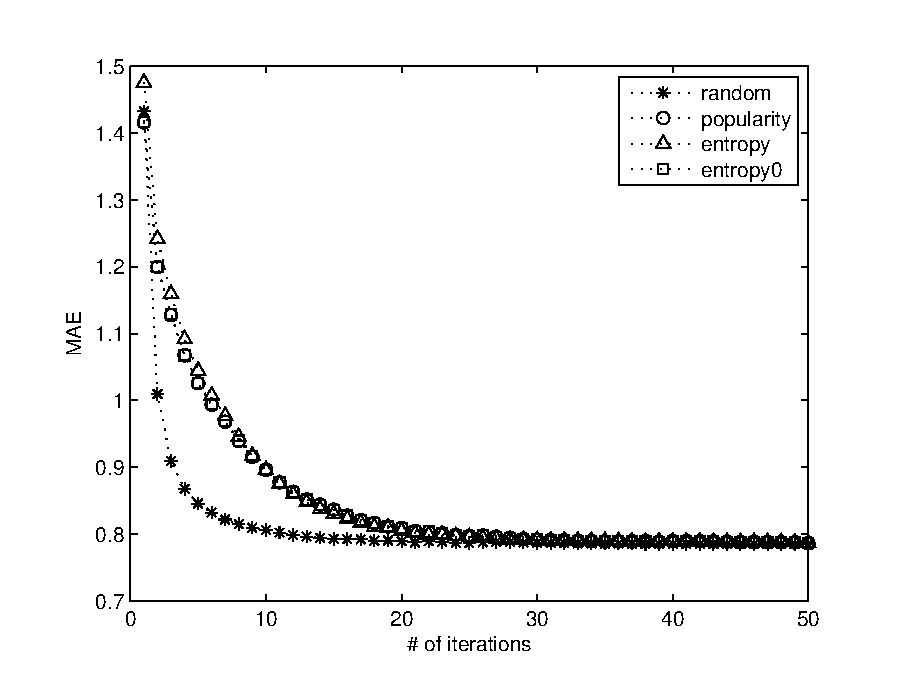
\includegraphics{ml_ent_ent0.eps}
\caption{Avaliação do grupo \textit{Entropia Pura} na base \textit{MovieLens}}
\label{fig:entropia-pura-movielens}
\end{figure}

\begin{figure}[ht]
\centering
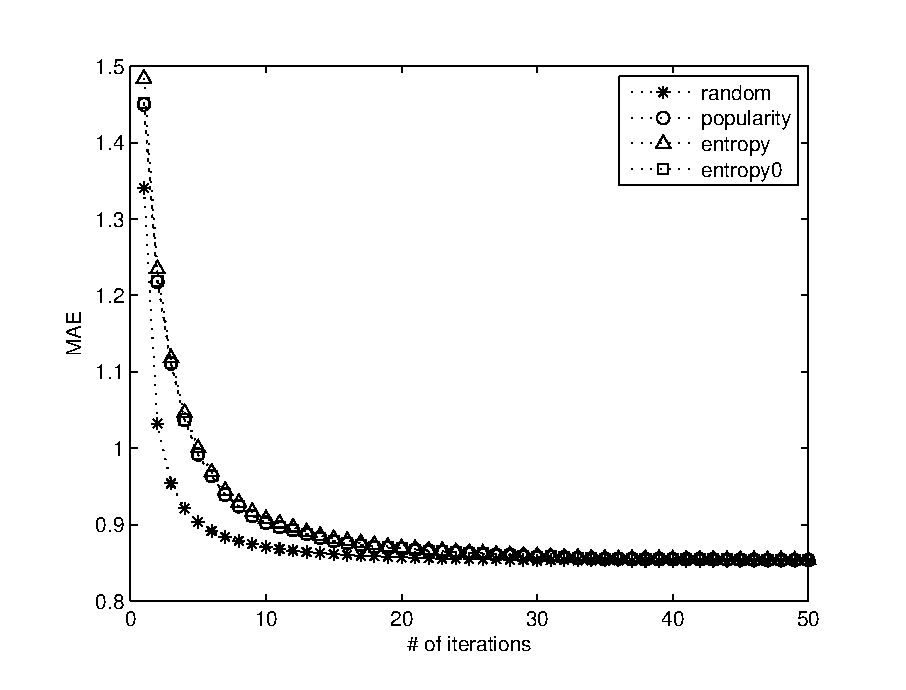
\includegraphics{nf_ent_ent0.eps}
\caption{Avaliação do grupo \textit{Entropia Pura} na base \textit{Netflix}}
\label{fig:entropia-pura-netflix}
\end{figure}

\subsection{Logaritmo da Popularidade e Entropia}

Do mesmo modo, as figuras \ref{fig:logpop-entropia-movielens} e \ref{fig:logpop-entropia-netflix} correspondem ao emprego de \textit{log(pop)*ent} e \textit{log(pop)*ent0} nas bases \textit{MovieLens} e \textit{Netflix}, respectivamente. Como é possível observar, ambas possuem comportamento muito similar a \textit{popularity}, entretanto havia indícios para suspeitarmos disso, uma vez que conhecemos os resultados do grupo \textit{Entropia Pura}.

Primeiramente, ambas estratégias estão baseadas no valor de popularidade, que representa o número de avaliações que o filme recebeu. Desta forma, tal valor, ainda que amenizado por uma função logarítmica, exerce forte influência sobre o comportamento da estratégia. Em segundo lugar, o outro componente que as compõe é o valor da entropia, dado pelas estratégias \textit{entropy} e \textit{entropy0}. É sabido que essas duas estratégias também não obtiveram comportamento muito destoante de \textit{popularity}. Logo, era esperado que tanto \textit{log(pop)*ent} como \textit{log(pop)*ent0} apresentassem comportamentos semelhantes à \textit{popularity}.

Fazendo uma analogia com o mercado de ações, podemos dizer que \textit{log(pop)*ent} está ``indexada'' por \textit{popularity} e \textit{entropy}, enquanto que \textit{log(pop)*ent0} está ``indexada'' por \textit{popularity} e \textit{entropy0}. Ou seja, assim como um fundo de investimento que está indexado por um determinado ativo (composto majoritariamente por este ativo) não apresentará rendimentos que destoam significativamente do rendimento deste ativo, da mesma maneira, o comportamento de tais estratégias não será muito distante do comportamento das suas estratégias ``índices''.

Em \citep{Elahi:2014:ALS:2542182.2542195} são apresentados apenas as estratégias \textit{log(pop)*ent} e \textit{popularity} e pode-se verificar que os comportamentos de ambas seguem bem próximos, o que confirma nossa analogia. 

\begin{figure}[ht]
\centering
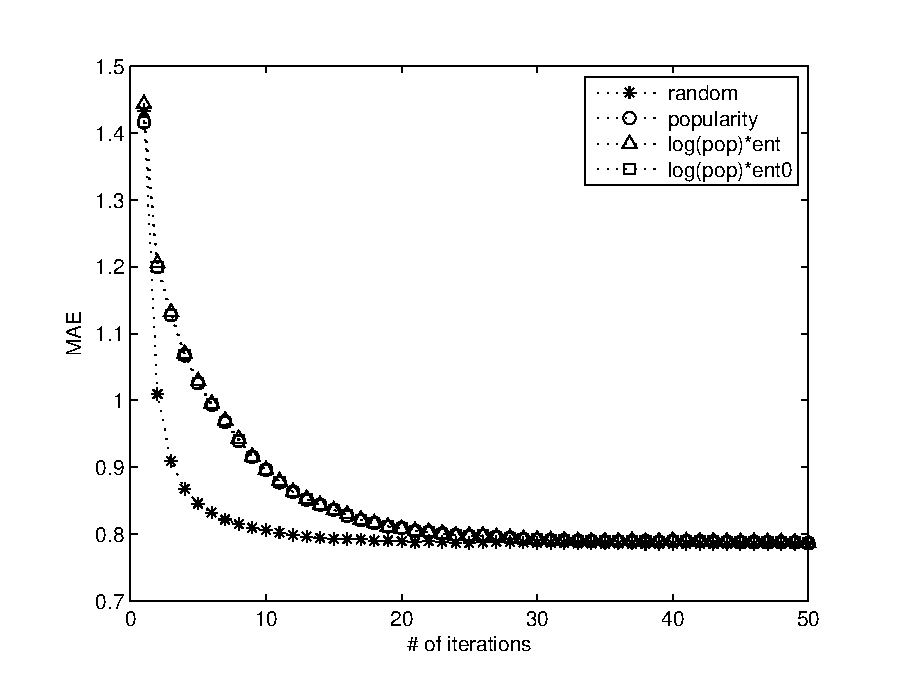
\includegraphics{ml_logpopent_logpop_ent0.eps}
\caption{Avaliação do grupo \textit{Logaritmo da Popularidade e Entropia} na base \textit{MovieLens}}
\label{fig:logpop-entropia-movielens}
\end{figure}

\begin{figure}[ht]
\centering
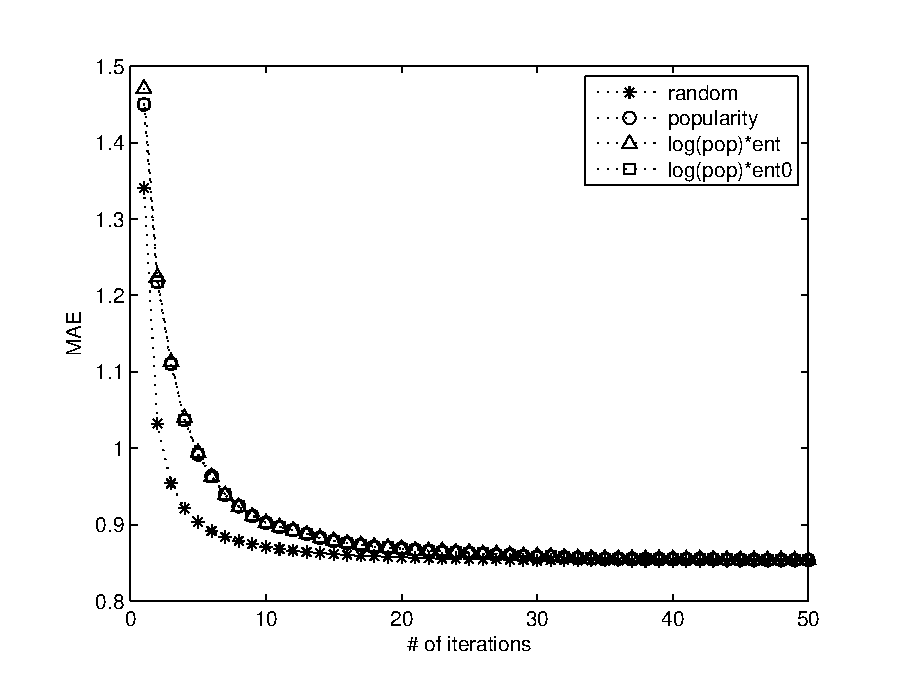
\includegraphics{nf_logpopent_logpopent0.eps}
\caption{Avaliação do grupo \textit{Logaritmo da Popularidade e Entropia} na base \textit{Netflix}}
\label{fig:logpop-entropia-netflix}
\end{figure}

\subsection{Média Harmônica da Popularidade e Entropia}

Novamente, pode-se observar a atração que as estratégias índices aplicam sobre suas indexadas. Vemos através das figuras \ref{fig:helf-movielens} e \ref{fig:helf-netflix} que \textit{helf} e \textit{helf0} recaem sobre \textit{popularity}. 

Este resultado, juntamente com o anterior, nos informa que tanto combinações simples (e.g., função logarítmica) como combinações complexas (e.g., média harmônica) não suprimem a atração que as estratégias compostas sofrem daquelas que as compõem. Concluímos então que a utilização de estratégias compostas, ou indexadas, não trará ganhos significativos quando as estratégias simples, as que lhes servem como índices, não possuem um bom comportamento elas mesmas.

Apesar de \citep{Elahi:2014:ALS:2542182.2542195} não fazer uso de \textit{helf} nem de \textit{helf0} em seus experimentos, os autores em \citep{Rashid:2008:LPN:1540276.1540302} apresentam os resultados que obtiveram com \textit{helf}. Conforme deduzido aqui, eles seguem bem próximos ao comportamento de \textit{popularity}. 

\begin{figure}[ht]
\centering
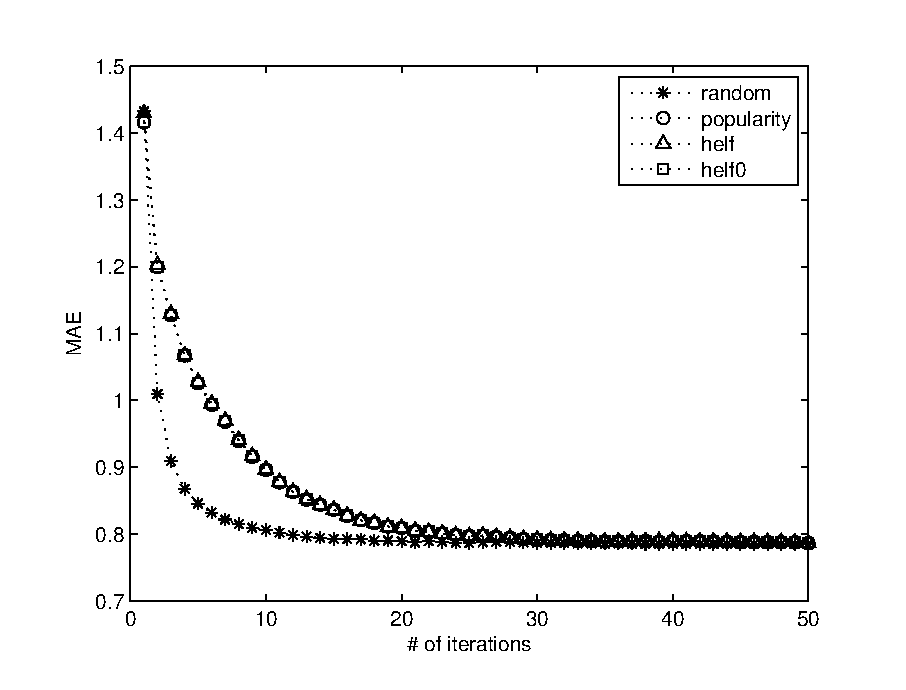
\includegraphics{ml_helf_helf0.eps}
\caption{Avaliação do grupo \textit{Média Harmônica da Popularidade e Entropia} na base \textit{MovieLens}}
\label{fig:helf-movielens}
\end{figure}

\begin{figure}[ht]
\centering
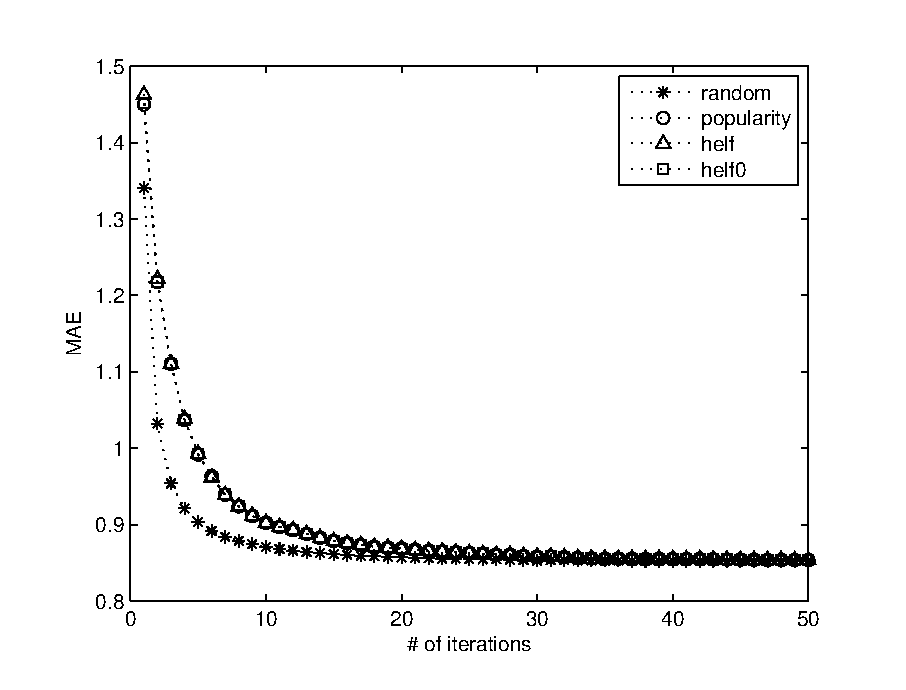
\includegraphics{nf_helf_helf0.eps}
\caption{Avaliação do grupo \textit{Média Harmônica da Popularidade e Entropia} na base \textit{Netflix}}
\label{fig:helf-netflix}
\end{figure}

\subsection{Ganho de Informação}

Dentre as estratégias da família \textit{Entropia}, \textit{igcn} parece ter obtido o melhor comportamento, conforme as figuras \ref{fig:igcn-movielens} e \ref{fig:igcn-netflix} indicam. Entretanto, mesmo sendo a melhor estratégia da família \textit{Entropia}, ela ainda fica muito aquém do desejado, que seria ultrapassar a estratégia \textit{random}.

Apesar de estar inserida nesta família, a \textit{igcn} não se baseia na entropia das preferências, mas sim na entropia dos usuários. Segundo \citep{Rashid:2008:LPN:1540276.1540302}, trabalho que propôs a estratégia, os usuários são divididos em grupos, chamados de \textit{clusters}, de acordo com suas disposições no espaço dado pela decomposição SVD. Os itens solicitados são aqueles que, se avaliados, reduzirão a incerteza associada a distribuição dos usuários em \textit{clusters}, i.e., trarão a maior redução na entropia da distribuição dos usuários.

Aqui, como no caso já comentado da entropia pura, há uma heurística subjacente à estratégia que parece introduzir viés no conjunto de treinamento. Buscar os itens com maior potencial para ``organizar'' os usuários, dentro de um espaço vetorial construído com base nas avaliações, não implica necessariamente em redução do erro do modelo. Afinal, é possível que o estado natural dos dados, incluindo as disposições dos usuários em tal espaço, seja um estado de desordem. Ao solicitar os itens que trarão uma maior organização, estamos induzindo uma ordem que é estranha aos dados e, consequentemente, podemos estar enviesando o conjunto de treinamento.

Somente \citep{Rashid:2008:LPN:1540276.1540302} apresenta resultados para \textit{igcn}, porém, infelizmente, não há comparações com \textit{random}. Todavia, faz-se comparações com \textit{helf}, \textit{entropy0} e \textit{popularity}, as quais se mostraram inferiores à \textit{igcn}, similar ao que foi verificado em nossos experimentos.

\begin{figure}[ht]
\centering
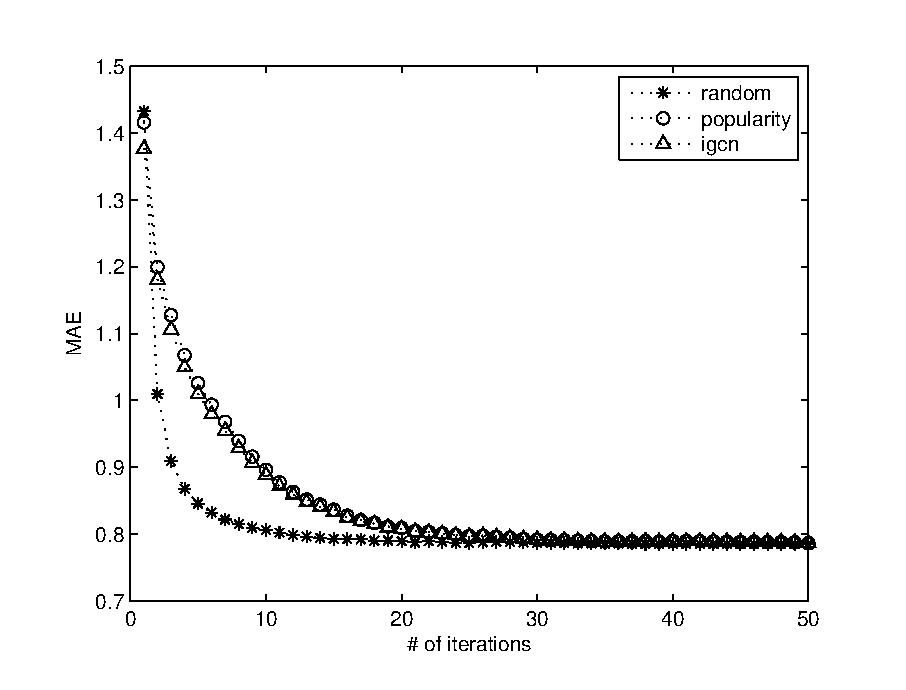
\includegraphics{ml_igcn.eps}
\caption{Avaliação do grupo \textit{Ganho de Informação} na base \textit{MovieLens}}
\label{fig:igcn-movielens}
\end{figure}

\begin{figure}[ht]
\centering
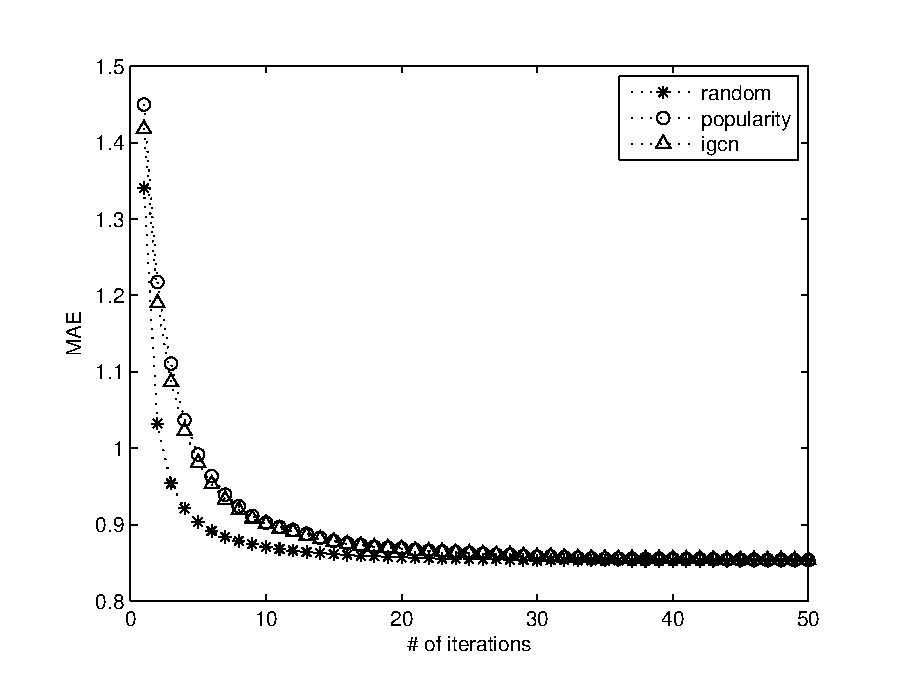
\includegraphics{nf_igcn.eps}
\caption{Avaliação do grupo \textit{Ganho de Informação} na base \textit{Netflix}}
\label{fig:igcn-netflix}
\end{figure}

\section{Variância}

Na família \textit{Variância}, como há apenas três estratégias, decidimos por não dividir em grupos e apresentá-las todas de uma só vez. Os resultados podem ser vistos nas figuras \ref{fig:variance-movielens} e \ref{fig:variance-netflix}, paras as bases \textit{Movielens} e \textit{Netflix}, respectivamente.

Vemos que a estratégias \textit{variance} apresenta uma ligeira vantagem sobre as demais, sobretudo na figura \ref{fig:variance-movielens}, nas primeiras 10 iterações. Contudo, seu comportamento passa logo a seguir o de \textit{popularity}, o que aponta para a presença de viés em $K$. Novamente, como no caso da entropia, tentar minimizar a incerteza dos itens através da variância, acarreta na construção de um conjunto de treinamento dominado pelos itens mais controversos. Tais itens são justamente os mais difíceis de se prever avaliações e, portanto, o modelo tem grande dificuldade em capturar o padrão que determina as avaliações dadas pelos usuários.  

As estratégias compostas utilizando \textit{variance} e \textit{popularity} caem no mesmo inconveniente das estratégias compostas que fazem uso de \textit{entropy} (ou \textit{entropy0}) e \textit{popularity}, ou seja, acabam por serem atraídas para o comportamento de \textit{popularity}. O que explica a semelhança de comportamento tanto de \textit{log(pop)*var} de \textit{sqrt(pop)*var} com \textit{popularity}.

\begin{figure}[ht]
\centering
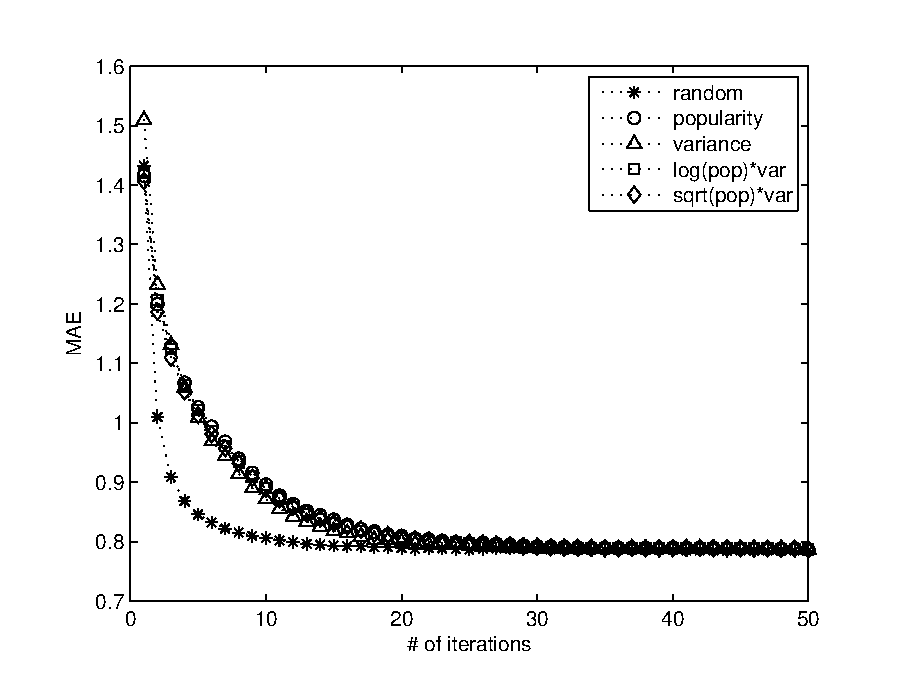
\includegraphics{ml_variance_family.eps}
\caption{Avaliação da família \textit{Variância} na base \textit{MovieLens}}
\label{fig:variance-movielens}
\end{figure}

\begin{figure}[ht]
\centering
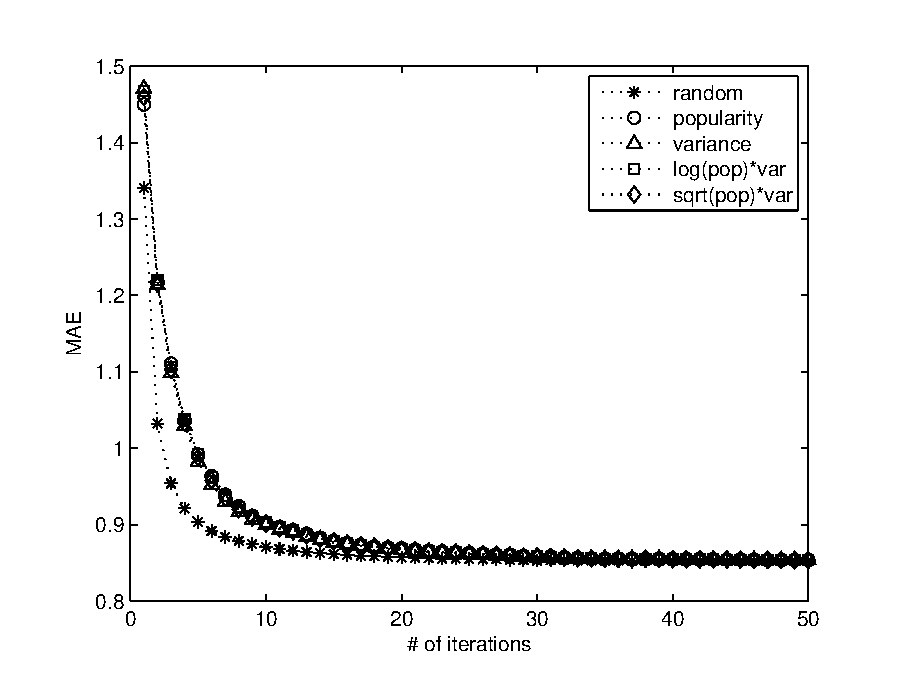
\includegraphics{nf_variance_family.eps}
\caption{Avaliação da família \textit{Variância} na base \textit{Netflix}}
\label{fig:variance-netflix}
\end{figure}

\section{Modelo}

Dentre as estratégias da família \textit{Modelo}, duas delas obtiveram desempenho pior que a estratégia \textit{random}, enquanto que as outras duas foram melhores. Aliás, deve-se mencionar que foram as únicas de todo nosso experimento que conseguiram tal feitio, com exceção da \textit{Estratégia Livre de Viés}. Cabe à nós então analisarmos o porquê deste comportamento inusitado, tendo sempre em mente a heurística por trás de cada estratégia.

\subsection{Pior que \textit{random}}

Começaremos por analisar as estratégias que obtiveram desempenho pior que \textit{random}, isto é, \textit{high pred} e \textit{bin pred}, exibidas nas figuras \ref{fig:worst-random-movielens} e \ref{fig:worst-random-netflix}. Observamos que ambas, até a 10ª iteração, apresentam desempenho ligeiramente superior à \textit{popularity}, convergindo mais tarde para o comportamento desta.

É importante levar em consideração que ambas as bases contêm preferências em forma de números inteiros, variando de 1 a 5. Das 100 mil avaliações presentes na base \textit{MovieLens}, cerca de 6\% das notas possuem valor igual a 1; 12\% igual a 2; 27\% igual a 3; 34\% igual a 4; e 21\% igual 5. Na base \textit{Netflix}, por sua vez, das 100 mil avaliações, cerca de 8\% possuem valor igual a 1; 14\% igual a 2; 35\% igual a 3; 27\% igual a 4; e 16\% igual a 5.

Se considerarmos as notas 1 e 2 como avaliações ``baixas'', e as notas 3, 4 e 5 como avaliações ``altas'', verificamos que \textit{MovieLens} e \textit{Netflix} possuem 82\% e 78\% das notas como sendo altas, respectivamente. Esta característica pode elucidar muito a respeito do desempenho que tais estratégias tiveram nessas bases.

A estratégia \textit{high pred} busca solicitar os itens que receberam as melhores previsões do modelo, ou seja, itens cujas previsões apontam para preferências altas. Desta maneira, ela insere no conjunto de treinamento $K$ sempre preferências altas, agravando o desequilíbrio natural que existe entre as preferências e tornando o conjunto ainda mais desbalanceado. Como o modelo é treinado com as preferências em $K$, este desequilíbrio transfere-se para a acurácia do mesmo, que acaba por ficar mais preciso em prever preferências altas do que baixas.

Por sua vez, \textit{bin pred} procura inserir em $K$ os itens cujas previsões apontam para alguma preferência, seja ela baixa ou alta. Em outras palavras, \textit{bin pred} solicita os itens cujas previsões indicam que os mesmos serão ``consumidos''. Esta abordagem não faz distinção entre as preferências, reduzindo-as a simples informações binárias. Com isso, acabamos simplesmente mantendo o desequilíbrio natural das preferências, visto que, ao contrário do caso de \textit{high pred}, não temos nenhuma ideia de como o usuário avaliará os itens solicitados.

Ambas as estratégias apresentam desempenho ruim em \citep{Elahi:2014:ALS:2542182.2542195}, ou seja, pior que \textit{random}. Contudo, no referido trabalho, \textit{bin pred} é nitidamente melhor que \textit{high pred}, o que não ficou claro em nossos experimentos. Na medida em que solicita apenas os itens de previsão alta, \textit{high pred} reforça o desequilíbrio entre as preferências em $K$, agravando a disparidade entre as previsões. Como \textit{bin pred} não sabe qual foi o valor efetivo da preferência prevista, o desequilíbrio em $K$ apenas se mantem com os itens solicitados. Por exemplo, mesmo que haja itens com previsão alta, é possível que \textit{bin pred} solicite itens com previsão baixa, o que não seria possível em \textit{high pred}.  

\begin{figure}[ht]
\centering
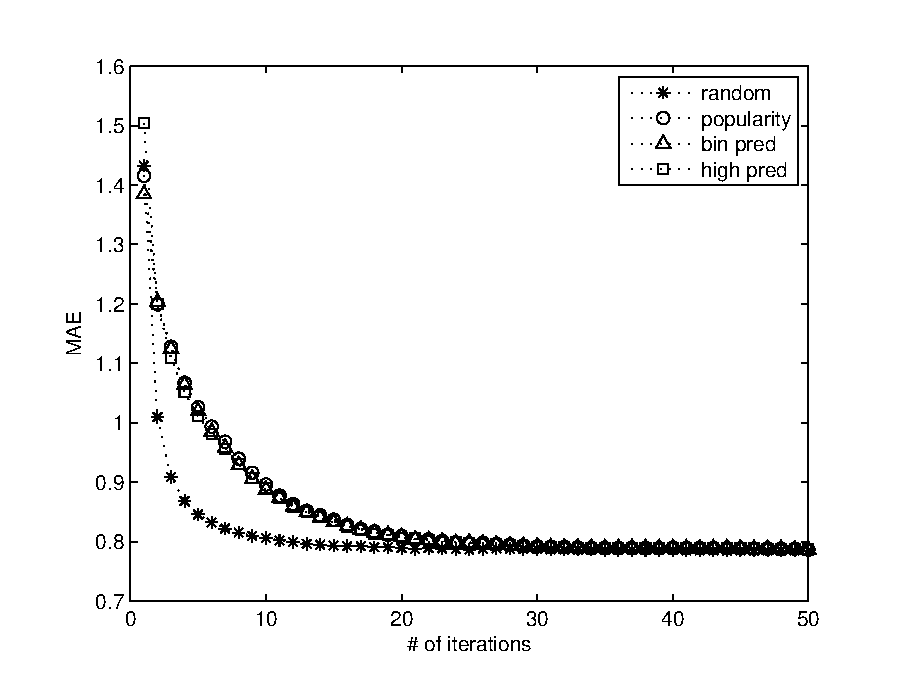
\includegraphics{ml_bin_high.eps}
\caption{Avaliação do grupo \textit{Pior que random} na base \textit{MovieLens}}
\label{fig:worst-random-movielens}
\end{figure}

\begin{figure}[ht]
\centering
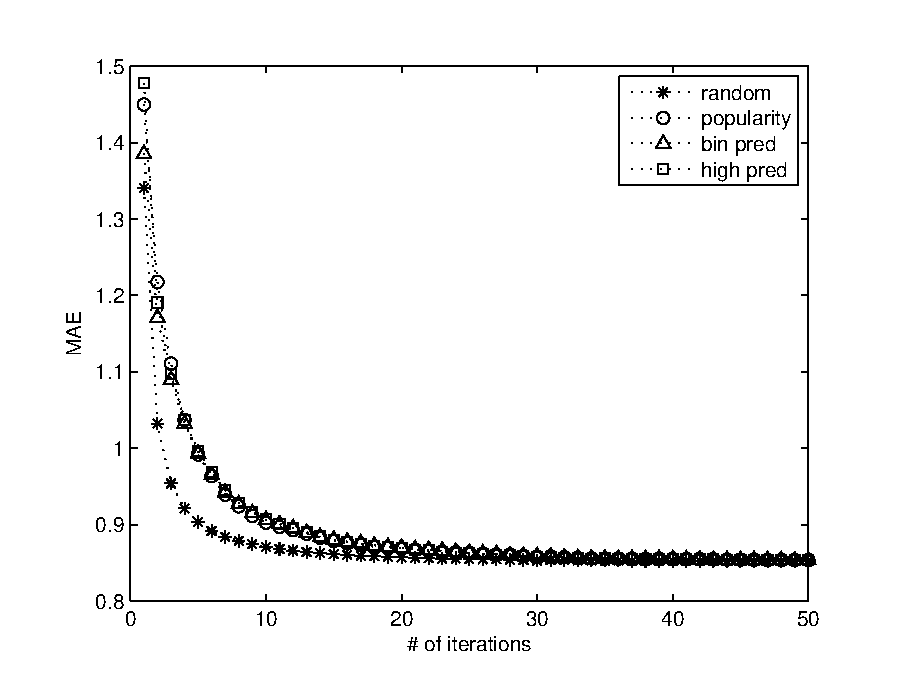
\includegraphics{nf_bin_high.eps}
\caption{Avaliação do grupo \textit{Pior que random} na base \textit{Netflix}}
\label{fig:worst-random-netflix}
\end{figure}

\subsection{Melhor que \textit{random}}
\label{sec:melhor-random}

As únicas estratégias que obtiveram desempenho melhor que \textit{random}, com exceção da \textit{Estratégia Livre de Viés}, foram \textit{low pred} e \textit{high-low pred}, conforme pode ser observado nas figuras \ref{fig:better-random-movielens} e \ref{fig:better-random-netflix}.

Ao contrário de \textit{high pred}, \textit{low pred} busca solicitar os itens cujas previsões apontam para preferências baixas. Uma vez que há uma carência natural por tais preferências, ao solicitá-las, esta estratégia introduz em $K$ justamente as preferências faltantes, amenizando o desequilíbrio entre preferências baixas e altas. O conjunto de treinamento acaba ficando mais equilibrado e, consequentemente, a acurácia do modelo fica mais balanceada, capaz de fazer previsões mais precisas para todos os tipos de preferência. 

Ou seja, a estratégia \textit{low pred} se beneficia da carência natural de preferências baixas. A heurística que a norteia, solicitar os itens com previsões baixas, mostrou-se eficaz visto que as bases utilizadas em nossos experimentos carecem de tais preferências. Caso as características das bases fossem outras ou se modificassem com o tempo, o desempenho da estratégia poderia ser diferente. Em outras palavras, o simples fato de que a estratégia obteve um bom desempenho não significa que ela não introduz viés no conjunto de treinamento. Pelo contrário, a própria concepção da estratégia implica na construção de um conjunto de treinamento enviesado, porém, neste caso, o viés nos foi útil.

Da mesma forma, \textit{high-low pred} assume que é preferível solicitar itens cujas previsões se distanciam do valor médio de preferência. Em ambas as bases, as avaliações podem possuir valores inteiros de 1 a 5, sendo o valor médio 3. Logo, \textit{high-low pred} procura solicitar itens cuja previsão é igual a 1 ou 5 (valores mais distantes do valor médio). Se definirmos as notas 1 e 5 como sendo avaliações ``extremas'' e as notas 2, 3, e 4 como avaliações ``medianas'', constatamos que 73\% das avaliações em \textit{MovieLens} são medianas, enquanto que, em \textit{Netflix}, este percentual é de 76\%.

Ou seja, a distinção entre avaliações baixas e altas esconde um pouco o verdadeiro desequilíbrio entre as preferências. Na verdade, as notas 3 e 4 compõem a grande maioria das avaliações nas duas bases, sendo 61\% das avaliações em \textit{MovieLens} e 62\% em \textit{Netflix}. Assim como \textit{low pred}, ao solicitar os itens cujas previsões apontam para preferências extremas, \textit{high-low pred} ameniza o desequilíbrio natural que existe nas bases e promove um treinamento mais balanceado do modelo. A heurística subjacente à estratégia acaba sendo, mais uma vez, útil, pois ataca justamente a desproporção entre as preferências. 

Em \citep{Elahi:2014:ALS:2542182.2542195}, tanto \textit{low pred} quanto \textit{high-low pred} apresentam desempenho pior que \textit{random} nas primeiras iterações, porém conseguem alcançar e superar esta estratégia. No entanto, \textit{high-low pred} mostrou-se melhor que \textit{low pred}, o que não ficou claro em nosso trabalho. Isto significa que a distinção entre preferências ``extremas'' e ``medianas'' representa melhor a realidade dos dados do que a distinção entre preferências ``baixas'' e ``altas''. 

%O bom desempenho de \textit{high-low pred}, por sua vez, pode ser explicado pelo mesmo argumento utilizado para justificar o desempenho das estratégias indexadas (e.g., \textit{helf}, \textit{log(pop)*ent0}, etc.). Isto é, como \textit{high-low pred} está indexada por \textit{low pred}, o comportamento da estratégia índice acaba por atrair o comportamento da indexada.
%O curioso de notar neste caso é que \textit{high-low pred} também está indexa por \textit{high pred}, que, por sua vez, não obteve um bom desempenho. Assim, temos motivos para supor que uma estratégia indexada por duas ou mais estratégias será atraída mais fortemente pela estratégia índice com melhor desempenho, contudo, maiores evidências se fazem necessárias para que possamos concluir de fato esta propriedade. Verificamos que \textit{low pred} e \textit{high-low pred} apresentam comportamentos semelhantes em \citep{Elahi:2014:ALS:2542182.2542195}, o que traz mais crédito à nossa análise.

\begin{figure}[ht]
\centering
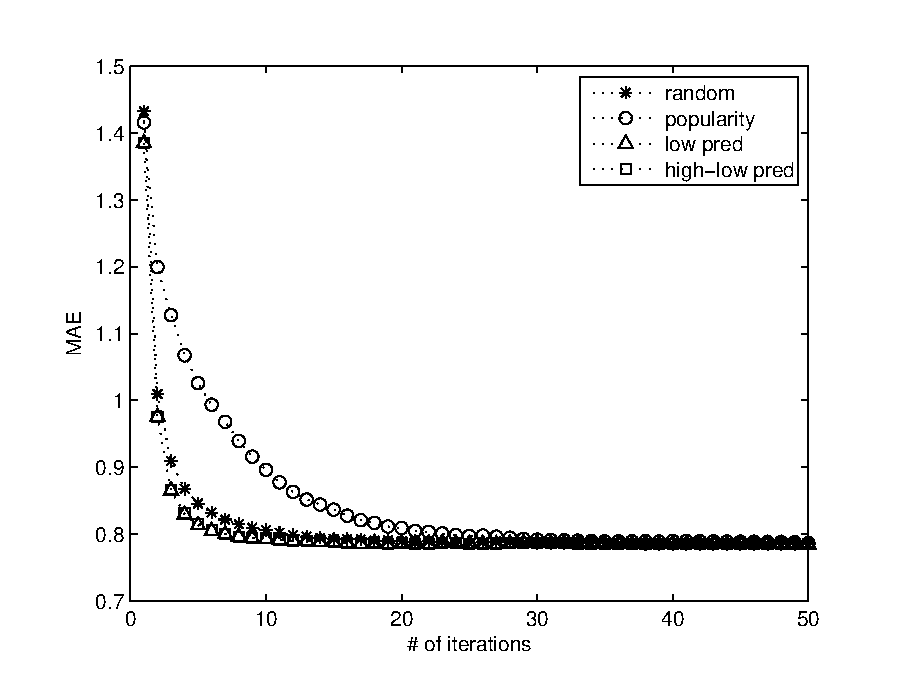
\includegraphics{ml_low_highlow.eps}
\caption{Avaliação do grupo \textit{Melhor que random} na base \textit{MovieLens}}
\label{fig:better-random-movielens}
\end{figure}

\begin{figure}[ht]
\centering
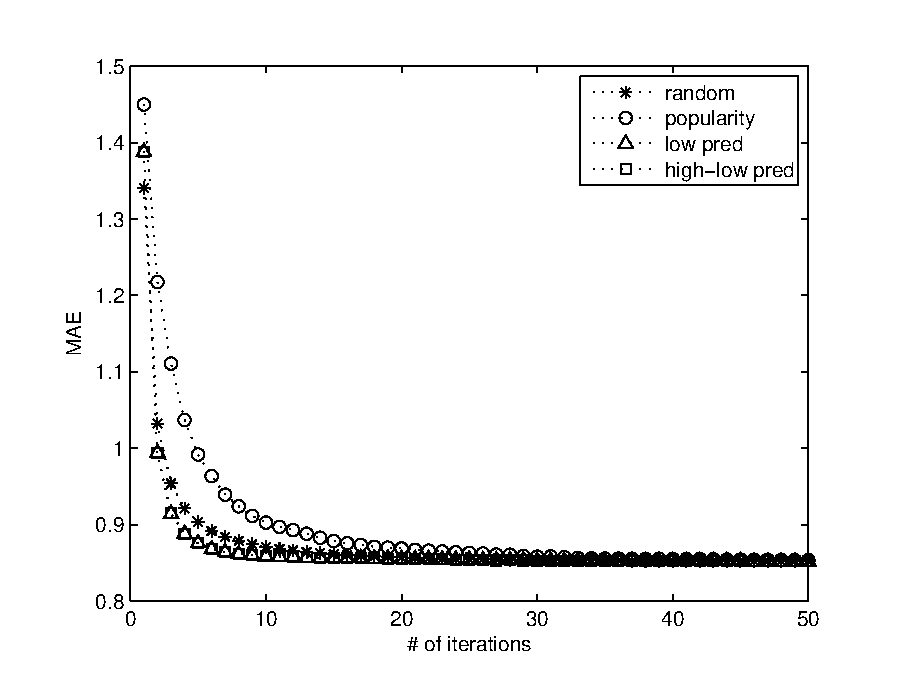
\includegraphics{nf_low_highlow.eps}
\caption{Avaliação do grupo \textit{Melhor que random} na base \textit{Netflix}}
\label{fig:better-random-netflix}
\end{figure}

\section{Estratégia Livre de Viés}

Iremos analisar nas próximas seções o comportamento da \textit{Estratégia Livre de Viés}, nomeada como \textit{unbiased} em nossos experimentos, comparando seu comportamento com as duas melhores estratégias até então: \textit{low pred} e \textit{high-low pred}. Além de uma análise global, visualizando todas as iterações, optamos também por realizar uma análise ampliada, com foco nas primeiras 15 primeiras iterações, onde é possível perceber mais nitidamente a superioridade de \textit{unbiased}.

\subsection{\textit{unbiased vs. low pred}}

As figuras \ref{fig:unbiased-lowpred-global-movielens} e \ref{fig:unbiased-lowpred-global-netflix} apresentam uma visão global, ou seja, uma visualização dos comportamentos de \textit{low pred} e \textit{unbiased} durante todas as iterações, nas bases \textit{MovieLens} e \textit{Netflix}, respectivamente. É possível verificar que, nas duas primeiras iterações, \textit{low pred} apresenta certa vantagem, entretanto, a partir da 3ª iteração, \textit{unbiased} parece alcançá-la e acompanhá-la até o final. Infelizmente, como o ganho de \textit{unbiased} é muito sutil, não conseguimos percebê-lo nesta escala.

Assim, decidimos por apresentar uma visão ampliada dos comportamentos de \textit{low pred} e \textit{unbiased}, até a 15ª iteração, de modo que seja possível visualizar com clareza a vantagem desta última. As figuras \ref{fig:unbiased-lowpred-focus-movielens} e \ref{fig:unbiased-lowpred-focus-netflix} exibem esta visão ampliada nas bases \textit{MovieLens} e \textit{Netflix}, respectivamente.

Vemos que \textit{unbiased} começa pior que \textit{low pred} em ambas as bases, porém, passadas algumas iterações, a primeira alcança a segunda e a supera. É interessante notar que, na base \textit{MovieLens}, \textit{unbiased} alcança \textit{low pred} já na 3ª iteração, enquanto que, em \textit{Netflix}, o empate só se dá por volta da 9ª iteração. Contudo, após o ponto de empate, em ambas as bases, pode-se observar que \textit{unbiased} toma a preeminência sobre a acurácia.

Um detalhe interessante é que esta preeminência de \textit{unbiased} é muito mais explícita na base \textit{MovieLens} do que na base \textit{Netflix}. Além do ponto de empate ocorrer mais cedo, o desvio padrão da acurácia, denotado pelas barras verticais, de \textit{unbiased} está abaixo do de \textit{low pred} em \textit{MovieLens} e eles não se sobrepõem. Isto significa que, mesmo no seu pior momento, o desempenho de \textit{unbiased} ainda é melhor do que o melhor momento de \textit{low pred}.

Embora este resultado nos remeta a conclusão de que \textit{unbiased} é efetivamente melhor que \textit{low pred}, é preciso lembrar que nossas conclusões devem se limitar ao dados em questão. Ou seja, apesar do comportamento de \textit{unbiased} ser nitidamente melhor que \textit{low pred}, na base \textit{MovieLens}, os resultados na base \textit{Netflix} já nos levam a uma conclusão diferente. Na média, o comportamento de \textit{unbiased} até foi superior ao de \textit{low pred} em \textit{Netflix}, no entanto, vemos que o desvio padrão das duas estratégias sobrepõem-se nesta base, o que indica que \textit{low pred}, em seus melhores momentos, pode superar \textit{unbiased}. 

Esta superioridade de \textit{unbiased} em \textit{MovieLens} pode ser explicada pelo fato de que a escolha dos parâmetros de \textit{unbiased} foi realizada com base apenas em \textit{MovieLens}. É possível que, utilizando parâmetros diferentes, possamos atingir resultados em \textit{Netflix} similares aos de \textit{MovieLens}. 

\begin{figure}[ht]
\centering
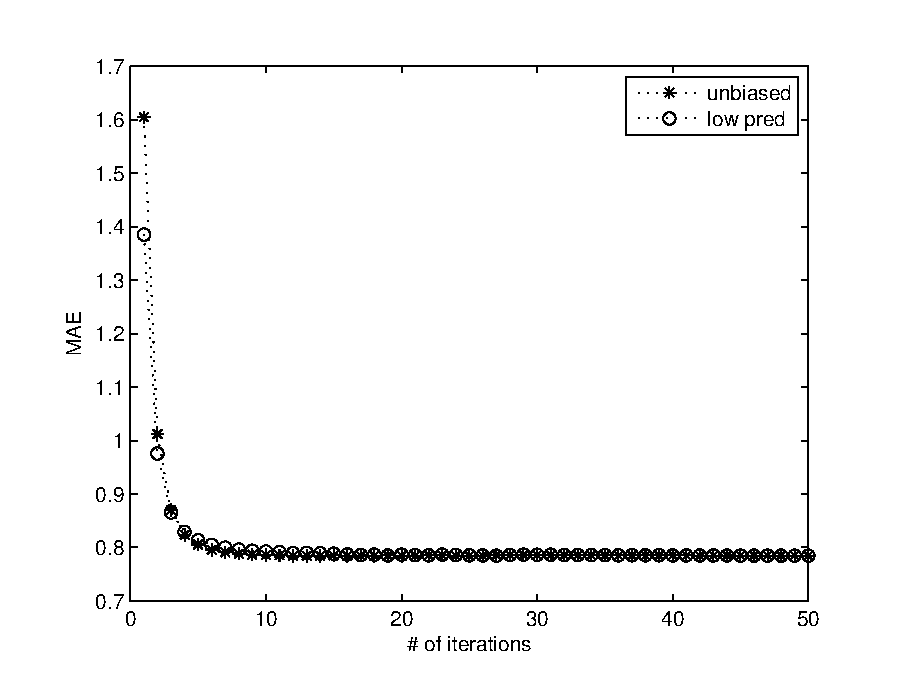
\includegraphics{ml_global_low_unbiased.eps}
\caption{Visão global de \textit{unbiased vs. low pred}  na base \textit{MovieLens}}
\label{fig:unbiased-lowpred-global-movielens}
\end{figure}

\begin{figure}[ht]
\centering
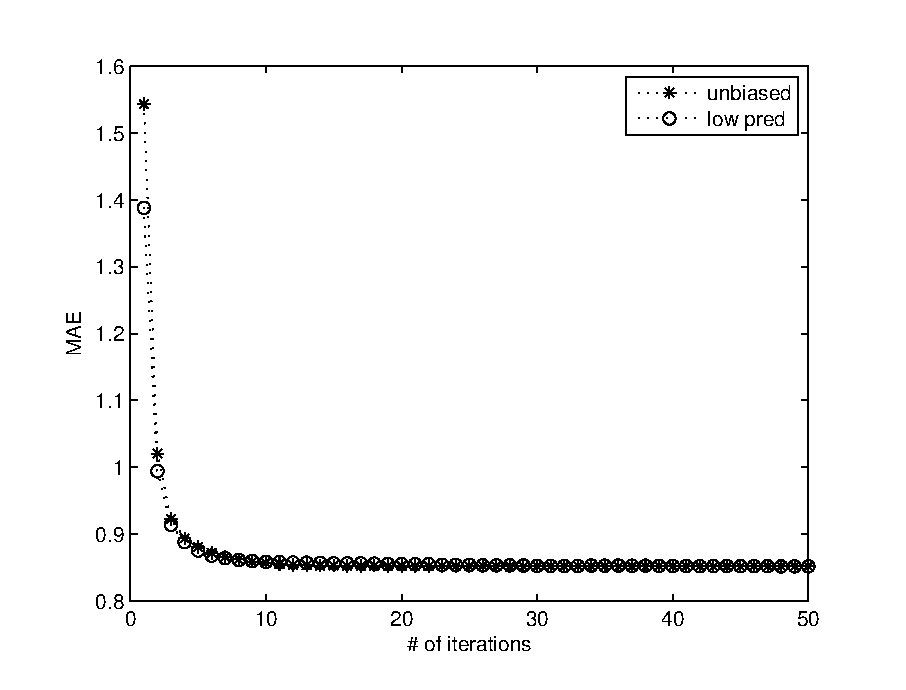
\includegraphics{nf_global_low_unbiased.eps}
\caption{Visão global de \textit{unbiased vs. low pred} na base \textit{Netflix}}
\label{fig:unbiased-lowpred-global-netflix}
\end{figure}

\begin{figure}[ht]
\centering
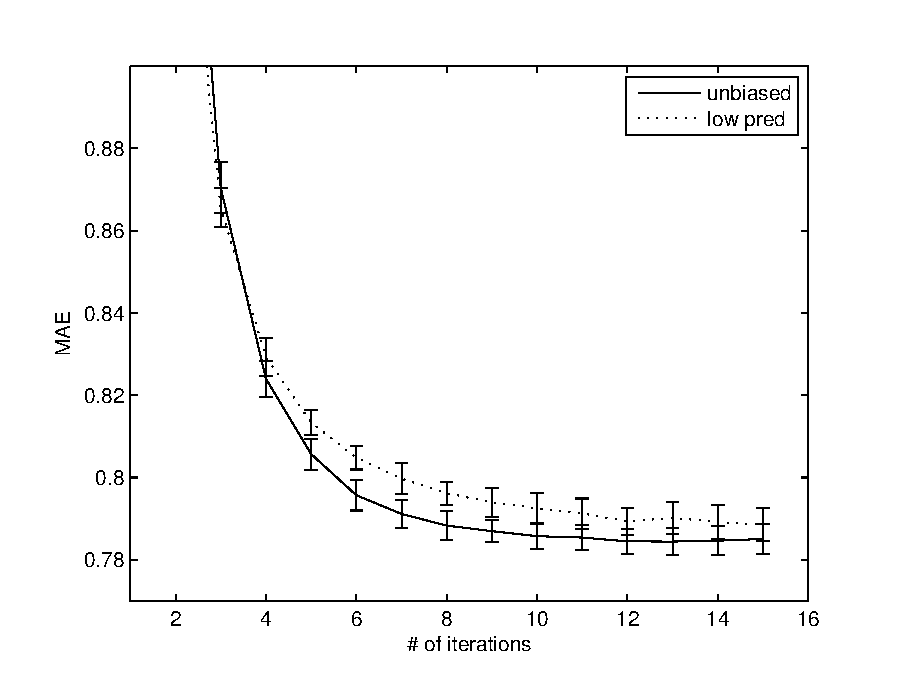
\includegraphics{ml_focus_low_unbiased.eps}
\caption{Visão ampliada de \textit{unbiased vs. low pred} na base \textit{MovieLens}}
\label{fig:unbiased-lowpred-focus-movielens}
\end{figure}

\begin{figure}[ht]
\centering
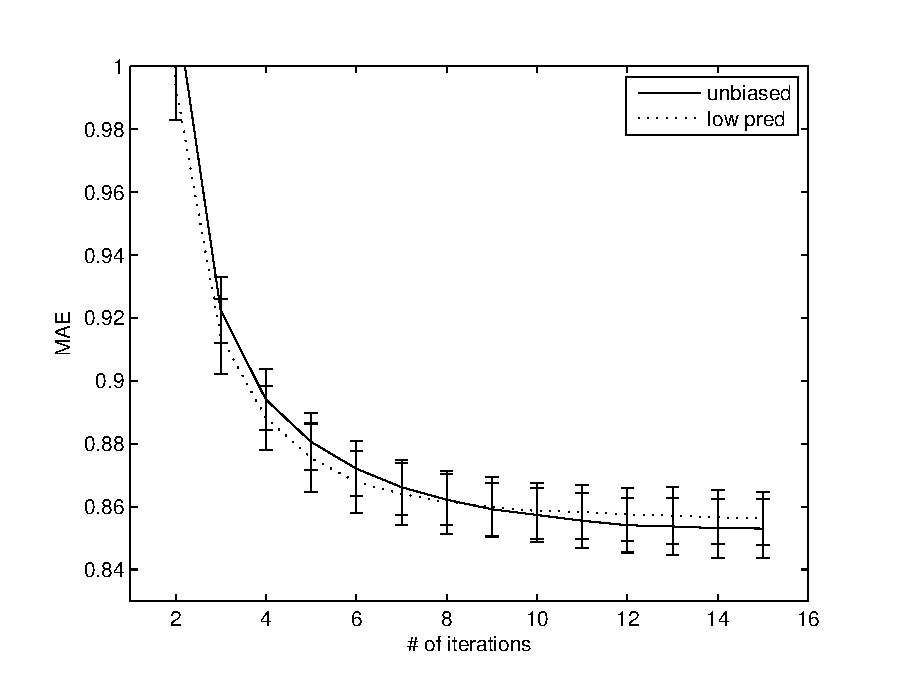
\includegraphics{nf_focus_low_unbiased.eps}
\caption{Visão ampliada de \textit{unbiased vs. low pred} na base \textit{Netflix}}
\label{fig:unbiased-lowpred-focus-netflix}
\end{figure}

\subsection{\textit{unbiased vs. high-low pred}}

Quando comparamos \textit{unbiased} com \textit{high-low pred} encontramos resultados muito parecidos com a comparação feita com \textit{low pred}. As figuras \ref{fig:unbiased-highlowpred-global-movielens} e \ref{fig:unbiased-highlowpred-global-netflix} exibem a visão global para as bases \textit{MovieLens} e \textit{Netflix}, respectivamente. Através delas, observa-se que, em ambas as bases, \textit{unbiased} começa com uma notória desvantagem frente a \textit{high-low pred}, porém, já na 3ª iteração, ambas parecem confluir para um mesmo valor e seguem assim até o final do experimento.

Na visão ampliada para as bases \textit{MovieLens} e \textit{Netflix}, obtida através das figuras \ref{fig:unbiased-highlowpred-focus-movielens} e \ref{fig:unbiased-highlowpred-focus-netflix}, respectivamente, vê-se que o ponto de empate de \textit{unbiased} e \textit{high-low pred}, em \textit{MovieLens}, se dá pela 3ª iteração, enquanto que, em \textit{Netflix}, este ponto se dá pela 9ª iteração. Além disso, a relação entre os desvios padrão também se mantem a mesma, já que em \textit{MovieLens} não há sobreposição e em \textit{Netflix} há.

De fato, não deveríamos esperar um resultado diferente para a comparação com \textit{high-low pred}. Tanto \textit{low pred} e \textit{high-low pred} se baseiam em heurísticas que procuram tornar o conjunto de treinamento mais balanceado. \textit{low pred} dá prioridade a itens com previsões 1 e 2 por serem avaliações ``baixas'', enquanto que \textit{high-low pred} também dá prioridade a itens com previsão 1 e 2 por serem ``extremas''. Assim, é esperado que haja uma enorme interseção dos itens solicitados por ambas as estratégias e, consequentemente, uma sintonia muito forte de seus comportamentos. Além disso, a questão dos parâmetros também influencia a obtenção do melhor resultado em \textit{MovieLens}.

\begin{figure}[ht]
\centering
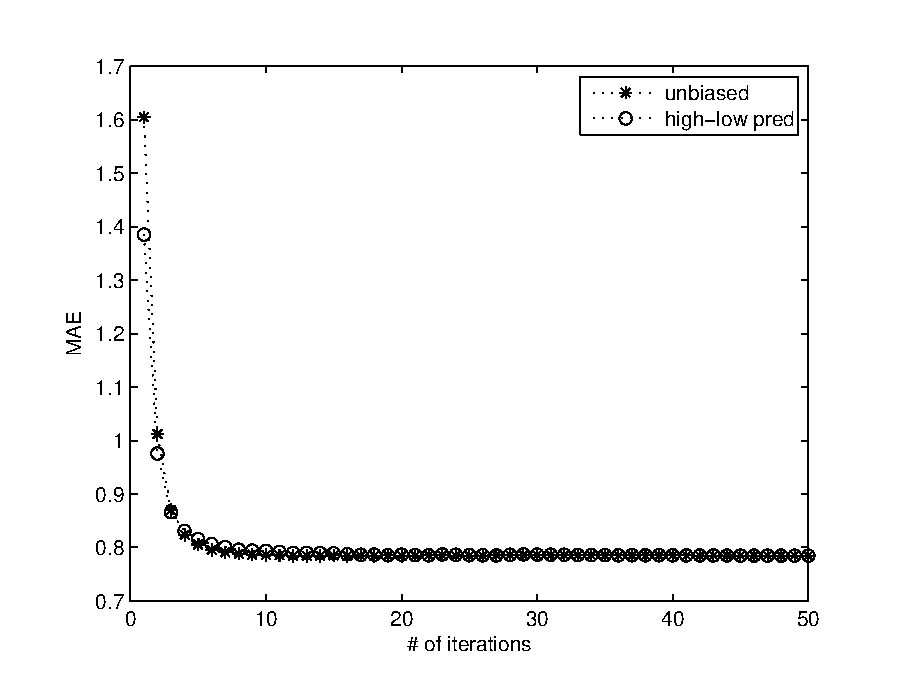
\includegraphics{ml_global_highlow_unbiased.eps}
\caption{Visão global de \textit{unbiased vs. high-low pred}  na base \textit{MovieLens}}
\label{fig:unbiased-highlowpred-global-movielens}
\end{figure}

\begin{figure}[ht]
\centering
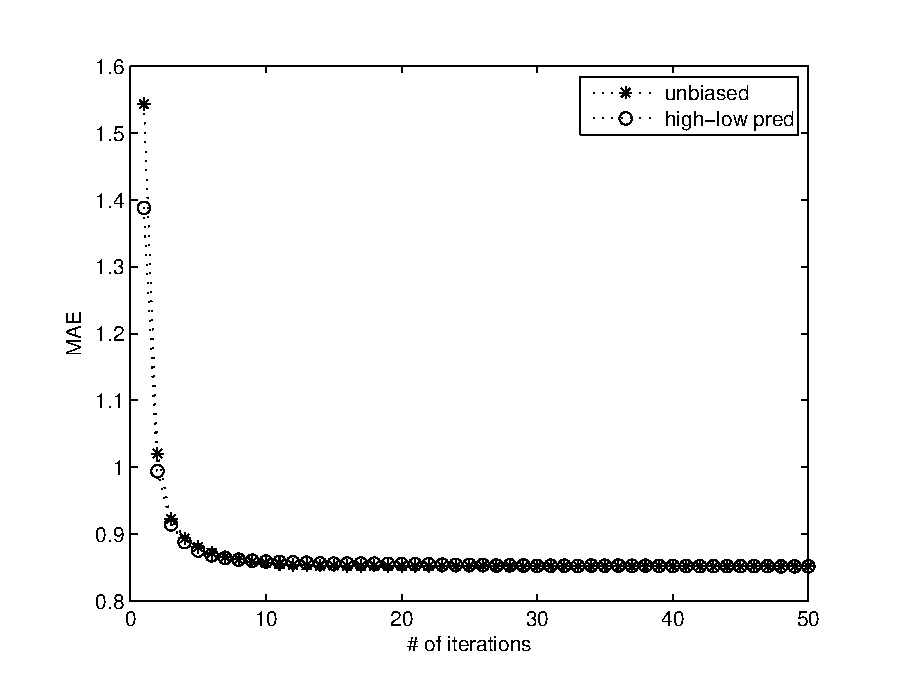
\includegraphics{nf_global_highlow_unbiased.eps}
\caption{Visão global de \textit{unbiased vs. high-low pred} na base \textit{Netflix}}
\label{fig:unbiased-highlowpred-global-netflix}
\end{figure}

\begin{figure}[ht]
\centering
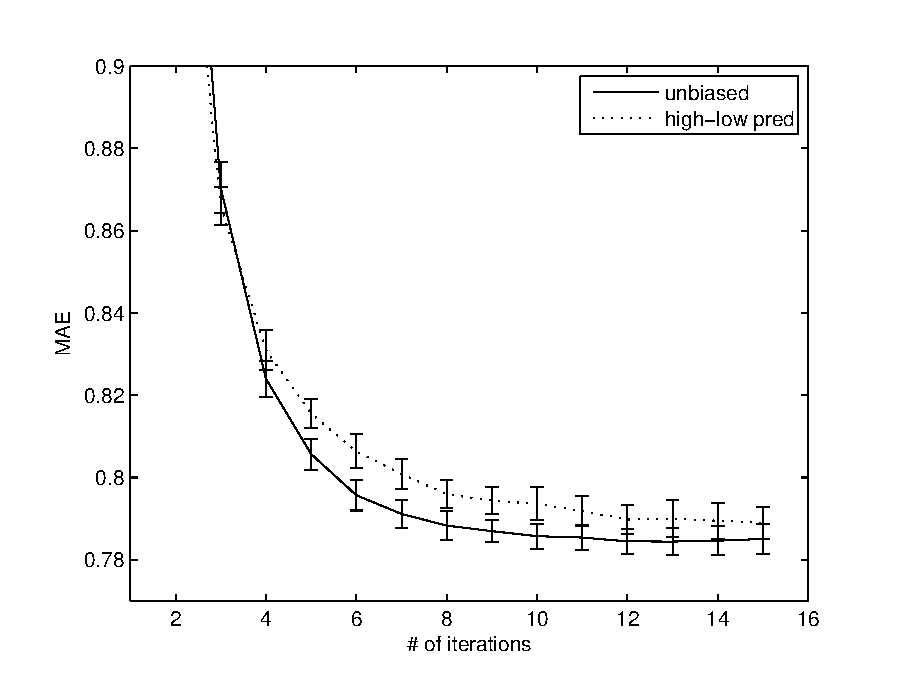
\includegraphics{ml_focus_highlow_unbiased.eps}
\caption{Visão ampliada de \textit{unbiased vs. high-low pred} na base \textit{MovieLens}}
\label{fig:unbiased-highlowpred-focus-movielens}
\end{figure}

\begin{figure}[ht]
\centering
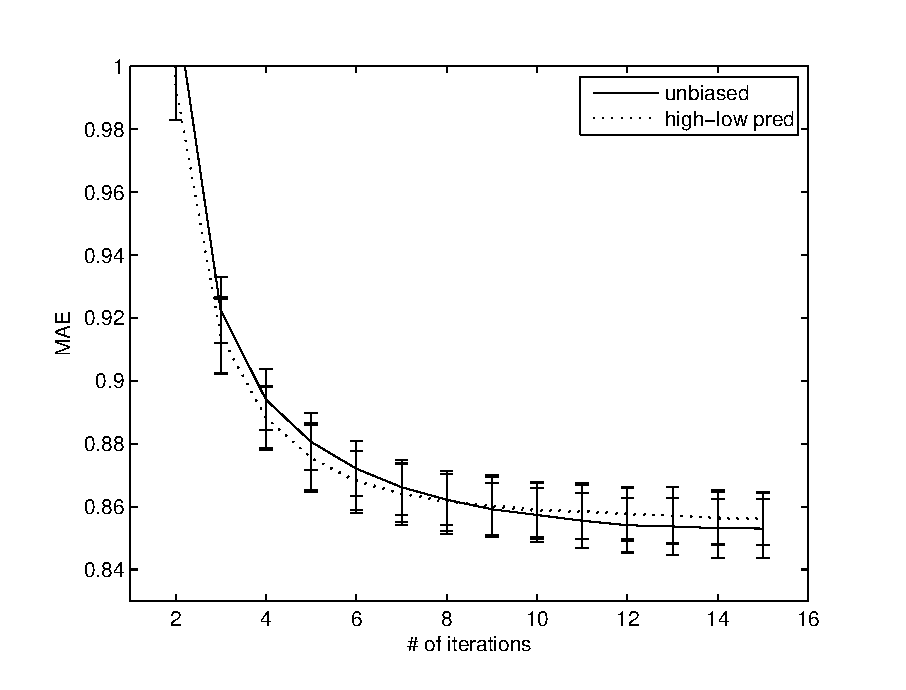
\includegraphics{nf_focus_highlow_unbiased.eps}
\caption{Visão ampliada de \textit{unbiased vs. high-low pred} na base \textit{Netflix}}
\label{fig:unbiased-highlowpred-focus-netflix}
\end{figure}
  \chapter{Conclusões e Trabalhos Futuros}
\label{cap:conclusao}

...

Como trabalhos futuros...


  \backmatter
  \bibliographystyle{coppe-unsrt}
  \bibliographystyle{thesis-real}
  \bibliography{thesis-real}

  %\appendix
  %\chapter{Algumas Demonstra{\c c}\~oes}

\end{document}
